% Document for printing A4 and 12pt fonts
\documentclass[a4paper,12pt]{book}
% We are using UTF8
\usepackage[utf8]{inputenc}
% The document is in English, but some text is also in Spanish
\usepackage[spanish,english]{babel}
% Math
\usepackage{amsmath,amsfonts,amssymb}
% Default fonts
\usepackage[T1]{fontenc}
\usepackage{slantsc}
\usepackage{microtype}
\usepackage{setspace}
\onehalfspacing
\usepackage{pxfonts}
\usepackage{varioref}
% Acronyms
\usepackage{acronym}
% Chapter headers
\usepackage[PetersLenny]{fncychap}
% Epigraphs
\usepackage{epigraph}
\usepackage{enumitem}
% Index
\usepackage{makeidx}
\makeindex
\newcommand{\idc}[1]{\index{#1@\texttt{#1}}\texttt{#1}}
\newcommand{\idx}[1]{\index{#1}{#1}}
\newcommand{\ida}[1]{\index{#1}{\ac{#1}}}
\newcommand{\idas}[1]{\index{#1}{\acs{#1}}}
\newcommand{\et}{\emph\&}
% Figures
\usepackage{graphicx}
\usepackage{wrapfig}
\graphicspath{{figures/}}
% Theme
\usepackage{fancyhdr}
% PDF with links
\usepackage[pdfusetitle,backref,colorlinks,linkcolor=blue]{hyperref}
% Uncomment to not use any colors in links (for printing)
%\hypersetup{colorlinks=false,pdfborder=0 0 0}
% Captions
\usepackage{caption}
% Code Listings
\usepackage{xcolor}
\usepackage{listing}
\usepackage{listings}
\DeclareCaptionFont{white}{\bfseries\sffamily\color{white}}
\DeclareCaptionFormat{listing}%
  {\colorbox{gray}{\parbox{\textwidth}{\hspace{14pt}#1#2#3}}}
\captionsetup[lstlisting]{format=listing,labelfont=white,textfont=white}
\definecolor{lightgray}{rgb}{.9,.9,.9}
\definecolor{darkgray}{rgb}{.4,.4,.4}
\definecolor{purple}{rgb}{0.65, 0.12, 0.82}
\lstdefinelanguage{JavaScript}{
  keywords={typeof, new, true, false, catch, function, return, null, catch,
  switch, var, if, in, while, do, else, case, break},
  keywordstyle=\color{blue}\bfseries,
  ndkeywords={class, export, boolean, throw, implements, import, this},
  ndkeywordstyle=\color{darkgray}\bfseries,
  identifierstyle=\color{black},
  sensitive=false,
  comment=[l]{//},
  morecomment=[s]{/*}{*/},
  commentstyle=\color{purple}\ttfamily,
  stringstyle=\color{red}\ttfamily,
  morestring=[b]',
  morestring=[b]"
}
\lstset{
  basicstyle=\ttfamily,
  flexiblecolumns,
  xleftmargin=18pt
}

%%%%%%%%%%%%%%%%%%%%%%%%%%%%%%%%%%%%%%%%%%%%%%%%%%
%%                   METADATA                   %%
%%%%%%%%%%%%%%%%%%%%%%%%%%%%%%%%%%%%%%%%%%%%%%%%%%
\title{Developing a Heavy Client-Side Web Application: ScaleNet}
\author{Víctor Pimentel Rodríguez}
\date{February 2011}
\hypersetup{pdfsubject=Proyecto Fin de Carrera}
%%%%%%%%%%%%%%%%%%%%%%%%%%%%%%%%%%%%%%%%%%%%%%%%%%

%%%%%%%%%%%%%%%%%%%%%%%%%%%%%%%%%%%%%%%%%%%%%%%%%%
%%               PAGE FORMATTING                %%
%%%%%%%%%%%%%%%%%%%%%%%%%%%%%%%%%%%%%%%%%%%%%%%%%%
\pagestyle{fancy}
\addtolength{\headwidth}{\marginparsep}
\addtolength{\footskip}{35pt}
\addtolength{\headwidth}{1.5cm}
\addtolength{\voffset}{-1cm}
\addtolength{\textheight}{1.5cm}
\addtolength{\hoffset}{-0.5cm}
\addtolength{\oddsidemargin}{0.9cm}
\addtolength{\paperheight}{1cm}

\fancyhf{}
\fancyhead[LE,RO]{\bfseries \thepage}
\fancyhead[LO]{\sffamily\scshape\footnotesize\rightmark}
\fancyhead[RE]{\sffamily\scshape\footnotesize\leftmark}

\newenvironment{abstract}{\cleardoublepage\null\vfill
  \begin{center}\Large\bfseries\abstractname\end{center}}{\vfill\null}
\newenvironment{acknowledgements}{\cleardoublepage\null\vfill
  \begin{center}\Large\bfseries{Acknowledgements}\end{center}}{\vfill\null}
%%%%%%%%%%%%%%%%%%%%%%%%%%%%%%%%%%%%%%%%%%%%%%%%%%

\begin{document}

%%%%%%%%%%%%%%%%%%%%%%%%%%%%%%%%%%%%%%%%%%%%%%%%%%
%%                     COVER                    %%
%%%%%%%%%%%%%%%%%%%%%%%%%%%%%%%%%%%%%%%%%%%%%%%%%%
\pagenumbering{alph}

\thispagestyle{empty}
\pdfbookmark{Title Page}{title}
\begin{titlepage}

  % Remove for the one-sided version
  \addtolength{\oddsidemargin}{0.45cm}

  \centerline{\large{\textls[50]{\textbf{\textsc{%
    Universidad Carlos III de Madrid}}}}}
  \vspace{0.8cm}

  \centerline{\large{\textls[50]{\textbf{\textsc{%
    Escuela Politécnica Superior}}}}}
  \vspace{0.8cm}

  \centerline{\large{\textls[50]{\textbf{\textsc{%
    Ingeniería en Informática}}}}}

  \begin{figure}[!htbp]
    \centering\includegraphics[height=2in]{logo-uc3m}
    %    \centering{\includegraphics[scale=1.3]{logo-uc3m-blue}}
    %    \centering{\includegraphics[scale=0.7]{logo-uc3m-wide}}
  \end{figure}

  \centerline{\Large{\textls[50]{\textbf{%
    \uppercase{PROYECTO FIN DE CARRERA}}}}}
  \vspace{2cm}

  \centerline{\textls[30]{\textbf{\textit{\huge{D}%
    \LARGE{EVELOPING A }\huge{H}\LARGE{EAVY }%
    \huge{C}\LARGE{LIENT-}\huge{S}\LARGE{IDE}}}}}
  \vspace{0.4cm}

  \centerline{\textls[30]{\textbf{\textit{\huge{W}\LARGE{EB }%
    \huge{A}\LARGE{PPLICATION: }%
    \huge{S}\LARGE{CALE}\huge{N}\LARGE{ET}}}}}
  \vspace{3.5cm}

  \begin{flushright}
      \begin{tabbing}\hspace{2.5cm} \= \kill
        {\large{\textls[30]{\textbf{Author}:}}} \>
        {\large{\textls[30]{\textbf{\textsc{Víctor Pimentel Rodríguez}}}}}\\
        {\large{\textls[30]{\textbf{Tutor}:}}} \>
        {\large{\textls[30]{\textbf{\textsc{Dr. José Ignacio
          Moreno Novella}}}}}\\
      \end{tabbing}
  \end{flushright}

  \begin{flushright}
    {\large{\textls[30]{\textbf{\textsc{March 2011}}}}}
  \end{flushright}

\end{titlepage}

\newpage
\thispagestyle{empty} \cleardoublepage

\begin{flushright}
  \null\vspace{\stretch{1}}
    {\textit{A mis padres y hermana: Inma, Julián y Sandra.}}\\
  \vspace{\stretch{1}}
    {\textit{(no me echéis de casa que ya me voy yo)}}
  \vspace{\stretch{2}}\null
\end{flushright}

\thispagestyle{empty}

\newpage
\thispagestyle{empty} \cleardoublepage
%%%%%%%%%%%%%%%%%%%%%%%%%%%%%%%%%%%%%%%%%%%%%%%%%%

%%%%%%%%%%%%%%%%%%%%%%%%%%%%%%%%%%%%%%%%%%%%%%%%%%
%%                  FRONTMATTER                 %%
%%%%%%%%%%%%%%%%%%%%%%%%%%%%%%%%%%%%%%%%%%%%%%%%%%
\frontmatter
\pagenumbering{roman}

\thispagestyle{empty}
\pdfbookmark{Resumen}{resumen}
\selectlanguage{spanish}
\begin{abstract}

Internet ha causado un tremendo impacto en muchos aspectos de nuestra vida cotidiana.
A medida que la sociedad se va acostumbrando a las facilidades de trabajar en línea, los hábitos cambian de manera acorde.
Aplicaciones que tradicionalmente se ejecutaban de manera nativa en la máquina del usuario se están, gradualmente, convirtiéndose en aplicaciones web ejecutadas remotamente.

Al mismo tiempo los navegadores han ido mejorando progresivamente hasta convertirse en potentes plataformas de desarrollo.
Esta mejora ha dado lugar a la aparición de aplicaciones web de una gran complejidad basadas en \idas{HTML}, \idas{CSS} y \idx{JavaScript}, distribuyendo una carga de procesamiento importante al cliente.
A la vez, se obtienen interfaces flexibles capaces de adaptarse a dispositivos muy dispares.

En este proyecto se documenta el desarrollo de una aplicación web avanzada cuyo propósito es controlar la reproducción de contenidos multimedia en varios dispositivos.
Esta aplicación se ha realizado en colaboración con \emph{Deutsche Telekom AG}, durante un estancia de seis meses en Berlín como parte del programa \emph{Erasmus Placement} en 2010.

Dicha aplicación se enmarca dentro del proyecto \idx{ScaleNet} (2005-2009), una Red de Siguiente Generación (\idas{NGN}) cuyo fin es un sistema que permita una integración escalable, rentable y eficiente de las diferentes tecnologías de acceso inalámbrico y por cable.
El componente desarrollado, la \emph{Interfaz de Administración de la Red Personal} (\idas{PNAI}), es solo una pequeña parte de \idx{ScaleNet} que sirve como ejemplo de aplicación sobre esta red.

Aunque la interfaz para estas operaciones ya existía, se solicitó un rediseño completo que integrara mayor funcionalidad y que ofreciera una experiencia de usuario más agradable.
Además de la interfaz principal para ordenadores de escritorio, también se explica el desarrollo de una interfaz web para dispositivos táctiles modernos.

\end{abstract}

\newpage
\thispagestyle{empty} \cleardoublepage

\thispagestyle{empty}
\pdfbookmark{Abstract}{abstract}
\input{front/abstract}
\newpage
\thispagestyle{empty} \cleardoublepage

\thispagestyle{empty}
\pdfbookmark{Acknowledgements}{acknowledgements}
\begin{acknowledgements}

I would like to thank my tutor José Ignacio for guiding me from Madrid, and Steffen, Dmitry and Hans for their warm welcome and constant help during my stay in Berlin.
Also thanks to T-Labs and the Erasmus Placement program for making this experience possible.

Thanks to Carolina, Javi, Laura, Lucas, Phillip and the rest of the friends that I made in Berlin, six months flew by because of their company.

Since this project culminates my studies in Universidad Carlos III, I also want to thank all the friends, colleagues and teachers that I met and that help me during all these years.
You made those endless hours working together in assignments seem bearable.

Finally, special thanks to my family for supporting me all these years and showing me all the patience in the world.

\begin{center}
  \line(1,0){250}
\end{center}

Me gustaría agradecer a mi tutor José Ignacio por orientarme desde Madrid, y a Steffen, Dmitry y Hans por su bienvenida y constante ayuda durante mi estancia en Berlín.
También agradecezo a los T-Labs y al programa Erasmus Placement el hacer posible esta experiencia.

Gracias a Carolina, Javi, Laura, Lucas, Phillip y al resto de amigos que hice en Berlín, por su compañía seis meses pasaron volando.

Dado que este proyecto culmina mis años de estudio en la Universidad Carlos III, también quiero agradecer a todos mis amigos, compañeros y profesores que he conocido y que me han ayudado durante todos estos años.
Habéis hecho fáciles de soportar las interminables horas trabajando juntos en prácticas.

Por último, un agradecimiento especial a mi familia por apoyarme todos estos años y por mostrarme toda la paciencia del mundo.

\end{acknowledgements}
\newpage
\thispagestyle{empty} \cleardoublepage

\pdfbookmark{Table of Contents}{contents}
\tableofcontents
\listoffigures
\listoftables
\listoflistings
\acresetall
%%%%%%%%%%%%%%%%%%%%%%%%%%%%%%%%%%%%%%%%%%%%%%%%%%

%%%%%%%%%%%%%%%%%%%%%%%%%%%%%%%%%%%%%%%%%%%%%%%%%%
%%                   MAINMATTER                 %%
%%%%%%%%%%%%%%%%%%%%%%%%%%%%%%%%%%%%%%%%%%%%%%%%%%
\mainmatter
\pagenumbering{arabic}

\chapter{Introduction and Objectives} % (fold)
\label{cha:introduction}

\setlength{\epigraphwidth}{11cm}
\renewcommand{\tabcolsep}{0em}

\epigraph{
\begin{tabular}{p{3cm}p{7.75cm}}
  \footnotesize{\textbf{\textsc{Michael Scott}} :}
    & I enjoy having breakfast in bed. I like waking up to the smell of bacon ---sue me--- and since I don't have a butler, I have to do it myself.\\
    & So most nights before I go to bed I will lay six strips of bacon out on my \emph{George Foreman} Grill.\\
    & Then I go to sleep.\\
    & When I wake up, I plug in the grill. I go back to sleep again.\\
    & Then I wake up to the smell of crackling bacon.\\
    & It is delicious. It's good for me. It's the perfect way to start the day.\\
    & Today I got up, I stepped onto the grill and it clamped down on my foot. That's it. I don't see what's so hard to believe about that. \\
\end{tabular}
\vspace{1em}
}{\textit{The Injury}\\ \textsc{The Office}}

\newpage

\section{Motivation} % (fold)
\label{sec:motivation}

The current document describes the work done under a Erasmus Placement internship in the \ida{T-Labs} of Berlin, developed during six months.
This department is in charge of several research projects regarding, mainly, next generation networks.

The \idx{ScaleNet} project was an attempt to converge several networks and services under the same system.
These services may include voice and video telephony, mobile TV, video on demand, online gaming and internet access.
Network convergence is seen as the migration of heterogeneous physical and logical network elements of fixed and mobile networks into one single (IP based) infrastructure.

This project was effectively finished in 2009, and one of the outcomes is an \ida{IMS} demonstration environment.
Using that demonstrator, service applications built on top of \idx{ScaleNet} are shown to companies and organizations that are potentially interested in the technology.

One of those applications is the \ida{PNAI} application, a web based \ida{GUI} from where the user can control running sessions in their devices.
Sessions are simply instances of the previously mentioned services, and they could be from phone calls to video streaming.

The system can manage any number of devices for each user, so he can register his mobile phone, laptop, desktop or TV and he can manipulate the sessions running in any device.
It has also some social capabilities implemented, so the user can also control a list of friends and can \emph{buy}, start, transfer or duplicate sessions for any of his friends.

Additionally, another web application called \idx{IPTVplus} is available to the user.
The purpose of this application is the acquisition of video content: live streaming, video on demand, etc.
The user can buy any content and a new session should automatically start on his default device.

The project motivation was improving the user interface by redesigning this \ida{PNAI}, implementing some functional extensions and integrating the \idx{IPTVplus} directly into the \ida{PNAI}.
With a little rethinking, the \ida{GUI} could be modernized so that the demonstrator were stunningly effective.

Later in the project, this task extended to porting the same functionality to a mobile web application to modern devices such as the \idx{iPhone}, the \idx{iPad} or the \idx{Android} devices.
The system only supported \emph{legacy} mobile devices like PDAs controlled by stylus, that were not really so sexy even back in their day.
% section motivation (end)
\nicesectionending
\section{Objectives} % (fold)
\label{sec:objectives}

The initial objective of the work was creating a modernized version of the \ida{PNAI} so that the interface were not only elegant but easy and fun to use.
As this work is for demonstrating the underlying technologies, things like efficiency or complete stability were not so important.

Even then, quality is always a welcomed addition, so a generic objective was developing a considerable sized \idx{JavaScript} application while maintaining a clear codebase.
That is not very easy to do with \idx{JavaScript}, so that impacted on the decision to use certain tools over others.

Also, the web application had to work on most browsers, but since we can control the demonstrator, we could reasonably drop some less used browsers if they could hinder the development.
Because of that, compatibility with \idx{Internet Explorer} 6 was dropped.

Giving that the \ida{PNAI} application is a little part of \idx{ScaleNet}, another goal was changing as less components as needed to avoid breaking other things.
This translates in no changes in the database, no changes in the messages and, even if one component -- the applet -- was replaced, the rest of the system does not even notice it.
Also, the deployment should be as simple as possible, the system already has a lot of dependencies.

As the project advanced, the goals evolved into filling other holes in the user experience.
Between them, the most important goal was unifying all functionality regarding sessions in one interface.
That is, to be able to buy content directly from the \ida{PNAI}, without having to go to other page first.

Another new objective was building a mobile web application compatible with \idx{iPhone} and other touch devices.
A mobile web application was chosen instead of a native app because that way the application is compatible with almost any device, and the web application will be faster to develop giving that most of the code can be recycled.
However, native applications feel \emph{better} than web pages, so that resulted in trying to mimic the experience of a native application in the mobile browser.

At the end of this document these objectives are evaluated to know if they were fulfilled, and at which level.
Additionally, some future goals are delineated for a plausible iteration over this work.
% section objectives (end)
\nicesectionending
\section{Project Phases} % (fold)
\label{sec:phases}

Since the beginning, the project had fairly unambitious objectives, so the timetable kept expanding based on feedback from the finished work.
According to the resulting development, the project can be structured in three phases, each of one taking a similar amount of time:

\begin{description}
  \item[Initial phase] To fulfill the original requirements, basically redesigning the \ida{PNAI} interface and adding some basic functionality relating the device list.
  In this phase all \idx{JavaScript} code was ported to \idx{MooTools} classes.
  \item[Intermediate phase] After that work was done, new requirements for the desktop version were added to implement more functionality into the \ida{PNAI} interface.
  Apart from creating a sidebar with the content list, the applet was replaced by the \ida{APE} server.
  This also includes fixing all kind of bugs with \idx{Internet Explorer}, working with the \ida{PHP} files and porting the existing \idx{Java} applet code to \idx{JavaScript}.
  \item[Final phase] The last goal in the project was creating the mobile version of the \ida{PNAI}.
  Also, this marks the transfer of the static files from the \ida{OSGi} bundle to the \ida{PHP} server.
\end{description}
% section phases (end)
\nicesectionending
\section{Document Structure} % (fold)
\label{sec:structure}

The work is mainly structured in four chapters, being this one the first.
In this chapter motivation and objectives for this project have been discussed, and the project phases have been delineated.

The second chapter explains the state of the art, that is, the existing technologies this project is based on.
This includes a somewhat detailed explanation of the \idx{ScaleNet} project in its current state, although only the relevant parts for this work have been reviewed.
Despite of the brevity of the existing documentation, some extra diagrams have been produced and added to help visualizing the system and more specifically the \ida{PNAI} interface.

Besides that system description, all the basic technologies used for the work are discussed, stating their utility and place in this work.
This sections talk about programming languages, platforms, libraries and techniques.

The third chapter concretes the actual development of this work, focusing on just the parts that have been modified.
New requirements are compiled and analyzed, producing use cases for all the new situations that need to be handled.
From that, the structure of the new system is described, starting from big components and going down to specific classes.

The development chapter continues with some implementation details that need further discussion or clarification.
The last section compiles the deployment instructions for upgrading a previous \idx{ScaleNet} installation to reckon the work in this project.

The four and last chapter evaluates this project, giving some conclusions to sum up the work made during those six months.
Also, it provides future insight and advice to possible directions expanding this project.

The end of this document collects an estimated budget, the bibliography used in this project, the definitions of the acronyms and an index of the key works.
% section structure (end)
\nicechapterending

% chapter introduction (end)
\chapter{State of the Art}

Bla bla bla

\section{Existing System: \idx{ScaleNet}} % (fold)
\label{sec:scalenet}

\idx{ScaleNet} \cite{SIE06} is a research project developed between 2005 and 2009.
Partly sponsored by the \emph{German Ministry of Education}, several major corporations participated, including \emph{Deutsche Telekom AG}, \emph{Alcatel SEL AG}, \emph{Eriksson GmbH}, \emph{Lucent Technologies} and \emph{Siemens AG}.
\ida{T-Labs} was specifically one of the departments more closely involved.

\begin{wrapfigure}{r}{0.5\textwidth}
  \centering
    \includegraphics[width=0.48\textwidth]{logo-scalenet}
  \caption{\idx{ScaleNet} logo}
  \label{fig:logo-scalenet}
\end{wrapfigure}

The aim of \idx{ScaleNet} is to provide a \ida{NGN} that integrates different wireless and wireline access technologies.
It is advertised as a scalable, cost effective and efficient \ida{FMC} solution.

\subsection{System Overview} % (fold)
\label{sub:overviewscalenet}

\idx{ScaleNet} addresses both service and network convergence.
At the lower level, the system supports a multitude of heterogeneous physical and logical network elements of fixed and mobile networks into one single all-IP infrastructure.
Figure~\ref{fig:scalenet-structure} lists some of the protocols that could be used~\cite{SIV08B}.

\begin{figure}[htbp]
  \centering
    \includegraphics[width=\textwidth]{scalenet-structure}
  \caption{Structure of the system}
  \label{fig:scalenet-structure}
\end{figure}

At a upper level, multimedia services relay on the \ida{IMS} framework for the delivery.
Theoretically \idx{ScaleNet} could support other protocols like Overlay Networks or \ida{P2P}, but \ida{IMS} is the one used by the current implementation.

It is important to notice that the own network is user-centric, and transparently handles identities by using \ida{SIP}.
This eases handling users with multiple devices; therefore applications do not have to worry about that part.

It is also important to define what a session means in this system.
A session refers to the current use of a service, so for every service that the user is enjoying a session is created.
For example, if it is viewing a movie but also talking on the \ida{IP} phone, there are two sessions at the same time.

The creation of a session implies that a new service is created, but it goes the other way around too.
If a session is deleted, that service must stop.
If the user ends the service, the session must be deleted.
That means sessions have to be synchronized with the actual services.

A session is also linked to the device that the user is using.
The system allows the copy and transfer of sessions to other devices that he owns, wherever it makes sense.
Since the current implementation has also basic social capabilities, that session can also be transferred or copied to a user's contact.
In the context of this application a user's contact is called ``buddy''.
Figure~\ref{fig:scalenet-structure} lists some of the services that can be offered:

\begin{itemize}
  \item Voice \et{} Video Calls
  \item Mobile TV \et{} \ida{VOD}
  \item \index{MMOG}\acp{MMOG}
  \item Internet Access
\end{itemize}

The work described in this document is primarily focused on the second application, i.e., video streaming.
The idea is that the user can buy a video and play it anywhere using any supported device.

% subsection overviewscalenet (end)

\subsection{\idx{IMS} Demonstrator} % (fold)
\label{sub:demonstrator}

\begin{figure}[p]
  \centering
    \includegraphics[width=\textwidth]{ims-arch}
  \caption{System architecture}
  \label{fig:ims-arch}
\end{figure}

\begin{figure}[p]
  \centering
    \includegraphics[width=\textwidth]{ims-arch-real}
  \caption{Architecture of the demonstrator}
  \label{fig:ims-arch-real}
\end{figure}

A logical view of the system is depicted in Figure~\ref{fig:ims-arch}, explaining the important nodes based on the capabilities needed.
The information relevant to this project is contained in the upper right corner of the figure, the nodes behind the control layer.

In the offices of \ida{T-Labs} in Berlin and Darmstadt there is a demonstrator with a working implementation of \idx{ScaleNet}.
That demonstrator is composed by several servers and a network infrastructure that enables access to the system using different network protocols and devices.
In Figure~\ref{fig:ims-arch-real} the actual network and hardware are exposed, replacing the same space as in the logical view (Figure~\ref{fig:ims-arch}).

\begin{figure}[htbp]
  \centering
    \includegraphics[width=\textwidth]{ims-setup}
  \caption{Setup of the demonstrator}
  \label{fig:ims-setup}
\end{figure}

Figure~\ref{fig:ims-setup} describes the setup in a better way and highlights the three different planes of the demonstrator.
The developed web application is executed from the \idx{Web Server} and the \idx{Application Server}, since it belongs to the service plane.
The signaling plane has also to be taken into account, because it communicates directly with the servers.

However, that is not the real deployment of the hardware used.
Whether for convenience or efficiency, tasks are distributed between two main servers.
This does not affect the logic of the system, since those tasks could be easily decoupled in an alternate deployment with more servers.
Anyway, the interesting pieces of hardware for this project are:

\begin{description}
  \item[\ida{IMS} core] This machine contains the \ida{IMS} server\footnote{The IMS core is open source software from Fraunhofer FOKUS and it can be freely downloaded from: \url{http://www.openimscore.org/}}, but since the \ida{IMS} load is not very high, it is responsible for other things.
  It acts as a \idx{Web Server} (using \idx{Apache} Web Server\footnote{\url{http://httpd.apache.org/}}) serving \idas{PHP} applications.
  It is also the internal \idas{DNS} server.
  \item[\idx{Application Server}] This is the \idas{IPTV} server, where the video content is streamed.
  It is also a \idx{Web Server}, but it serves \idx{Java} applications based on the \idas{OSGi} framework\footnote{\url{http://www.osgi.org/}}.
  \item[User Devices] Devices intended for the user to access the services.
  There is a TV, a laptop and several phones.
  All of them run a custom \ida{IMS} client that holds a connection to the servers, allowing the identification and adding \idas{IPTV} and \idas{VoIP} capabilities to those devices.
  In the last phase of the development, an \idx{iPhone} was added for testing purposes.
\end{description}

This demonstrator contains several demo applications running.
The interesting one for this project is the application that handles \idas{IPTV} streaming.

% subsubsection stoppingplayback (end)

\subsection{Personal Network Administration Interface (\idx{PNAI})} % (fold)
\label{sub:pnai}

The Web interface used for the management of sessions is called \ida{PNAI}~\cite{SIV08A}. From this interface the user can obtain this information:

\begin{itemize}
  \item All devices and registered in the system for that user and their online status.
  \item All buddies for that user and their online status.
  \item All multimedia sessions related to the user. This includes:
  \begin{itemize}
    \item The sessions running on his devices, no matter who paid for that content.
    \item The sessions running on devices from his buddies and started/paid by that user.
  \end{itemize}
\end{itemize}

Those are passive actions, but from that same view the user can initiate some operations to control the system.
In Figure~\ref{fig:usecasesiptv} all the available operations relating sessions are listed following a use case diagram.

\begin{figure}[htbp]
  \centering
    \includegraphics[width=\textwidth]{diagrams/usecases-pnai-old.1}
  \caption{Use cases for the IPTV application}
  \label{fig:usecasesiptv}
\end{figure}

In that diagram colors are used to differentiate the different kind of use cases covered. Also two visual marks (* and **) are added in case this is a copy in black a white. The meaning of the colors are explained according to this legend:

\begin{description}
  \item[Green] Available already in the main \ida{PNAI} page.
  \item[Purple (\emph{marked with *})] Available in an individual page outside of the main \ida{PNAI} page.
  \item[Red (\emph{marked with **})] Not implemented.
\end{description}

As we can see, the main \ida{PNAI} page has already a lot of functionality, but it can contain even more. Basically the actions available to that user in that page are:

\begin{itemize}
  \item Terminate a session of a user device or of a buddy if the session is owned by that user.
  \item Transfer (handover) or copy (duplication) a existing session to a user device or to a buddy if the session is owned by that user. That is, if one buddy bought the content for us, we cannot transfer again that content to another buddy.
\end{itemize}

Beside of these session related operations, there are other management operations.
For example, selecting which device is the default, adding/removing devices or adding/removing buddies.
For this document they are not relevant since they remained untouched.

Figure~\ref{fig:pnai-old} shows the old appearance of the main page for a logged user, before any work began.
On the left side of the page there is the \idx{Device List}, where the devices owned by that user are drawn.
On the right side there is the \idx{Buddy List}, where the user's buddies are listed.
Finally, the trash bin is in the lower right corner of the \idx{Device List}. 

\begin{figure}[htbp]
  \centering
    \includegraphics[width=\textwidth]{pnai-old}
  \caption{Old \idas{PNAI} page}
  \label{fig:pnai-old}
\end{figure}

The devices that are offline are disabled and are drawn with a dimmed appearance.
The buddies that are online are preceded by a green icon, while the ones that are offline are preceded by a red icon.

Devices or buddies that are online act as session containers.
The reason for the devices to be so big is because inside them the current sessions are drawn.
Besides the name of the content playing, session have an icon that changes depending on the type of session (video, audio, call, etc).

The user can interact with the sessions through the mouse using drag\et{}drop.
For example, the user can \emph{grab} the icon he wants and drop it in another container to copy or transfer that session.
That is a very visual and fast way to manage sessions.

When a user drops the session in another container, a menu will appear to ask the user if he wants to copy or transfer that session.
The trash bin acts also as a container, but in a special way: when a session is dropped in the trash bin, that session is automatically deleted, with no menu involved.

\subsubsection{Use Cases} % (fold)
\label{ssub:usecasesold}

\begin{center}
  \begin{usecase}[Stop a session of a device]
    \label{tab:usecasestopdevice}%
    \usecaseactor{System user}
    \usecasepre{A session is already running on a device, and it is showing in the \ida{PNAI} interface inside of that device.}
    \usecasepost{Session must terminate, i.e., the content must stop playing. The user must be notified with a popup and the session icon must be deleted from the \ida{PNAI} interface.}
    \usecasemain{
      \begin{usecasepath}
        \item User starts dragging the session icon.
        \item A copy of the session icon appears under the user's cursor, and follows the cursor until the user drops it.
        \item User drops the cloned session icon into the trash.
        \item A popup appears to notify the user that the action is in progress and the cloned session icon is deleted from the view.
        \item The content stops playing.
        \item The popup disappears and the original session icon is deleted from the view.
      \end{usecasepath}
    }
    \usecasealt{1}{
      \begin{usecasepath}[b]
        \setcounter{enumi}{2}
        \item User drops the session into a blank space.
        \item Action is cancelled.
      \end{usecasepath}
    }
    \usecasealt{2}{
      \begin{usecasepath}[c]
        \setcounter{enumi}{4}
        \item There is an error with the server and the content keeps playing.
        \item The content of the popup changes to notify the user that there was an error with the server and the action could not be completed.
        After 5 seconds it disappears.
        \item Action is cancelled.
      \end{usecasepath}
    }
    \usecasealt{3}{
      \begin{usecasepath}[d]
        \item There is an error with the server and the content keeps playing.
        \item The content of the popup changes to notify the user that there was an error with the server and the action could not be completed.
        After 5 seconds it disappears.
        \item Action is cancelled.
      \end{usecasepath}
    }
  \end{usecase}
\end{center}

The use case for terminating a session that a buddy is playing and that we own is very similar:

\begin{center}
  \begin{usecase}[Stop a session of a buddy]
    \label{tab:usecasestopbuddy}%
    \usecaseactor{System user}
    \usecasepre{A session owned by the user is running on a device, and it is showing in the \ida{PNAI} interface near that buddy's name.}
    \usecasepost{Session must terminate, i.e., the content must stop playing. The user must be notified with a popup and the session icon must be deleted from the \ida{PNAI} interface. The buddy is \emph{not} notified, the content stops without warning.}
    \usecasemain{
      \begin{usecasepath}
        \item User starts dragging the session icon.
        \item A copy of the session icon appears under the user's cursor, and follows the cursor until the user drops it.
        \item User drops the cloned session icon into the trash.
        \item A popup appears to notify the user that the action is in progress and the cloned session icon is deleted from the view.
        \item The content stops playing.
        \item The popup disappears and the original session icon is deleted from the view.
      \end{usecasepath}
    }
    \usecasealt{1}{
      \begin{usecasepath}[b]
        \setcounter{enumi}{2}
        \item User drops the session into a blank space.
        \item Action is cancelled.
      \end{usecasepath}
    }
    \usecasealt{2}{
      \begin{usecasepath}[c]
        \setcounter{enumi}{4}
        \item There is an error with the server and the content keeps playing.
        \item The content of the popup changes to notify the user that there was an error with the server and the action could not be completed.
        After 5 seconds it disappears.
        \item Action is cancelled.
      \end{usecasepath}
    }
  \end{usecase}
\end{center}

% subsubsection usecasesold (end)

\subsubsection{Class Diagrams} % (fold)
\label{ssub:classdiagramsold}

\begin{figure}[htbp]
  \centering
    \includegraphics[width=\textwidth]{diagrams/class-pnai-js-old.1}
  \caption{Class diagram for the old \idas{PNAI}}
  \label{fig:classdiagramsold}
\end{figure}

\begin{figure}[htbp]
  \centering
    \includegraphics[width=\textwidth]{diagrams/component-pnai-old.1}
  \caption{Component diagram for the old \idas{PNAI}}
  \label{fig:componentdiagramsold}
\end{figure}

\begin{figure}[htbp]
  \centering
    \includegraphics[width=\textwidth]{diagrams/sequence-handover-old.1}
  \caption{Sequence diagram for the old \idas{PNAI}}
  \label{fig:handoverscenarioold}
\end{figure}

% subsubsection classdiagramsold (end)
% subsection pnai (end)

\subsection{IPTVplus} % (fold)
\label{sub:iptvplus}

From the main \idas{PNAI} page the user can control the sessions that are already created but, how can he create new sessions?
Another page called \idx{IPTVplus} lists all the multimedia services available to the user in categories, with thumbnails, descriptions, prices and buttons to buy that content.
Figure~\ref{fig:iptvplus} shows how the page looks.

\begin{figure}[htbp]
  \centering
    \includegraphics[width=\textwidth]{iptvplus}
  \caption{Old IPTVplus page}
  \label{fig:iptvplus}
\end{figure}

Basically, the user clicks on the button \textit{Start} to buy a content, then a popup appears to confirm the selection.
If confirmed, the user is \textit{charged} and the content starts playing in his default device.

For the user perspective this could be handled more elegantly, since the functionality is split between \idx{IPTVplus} and the \idas{PNAI}.
One of the goals of this work is integrating that functionality directly in the main \idas{PNAI} page.

% subsection iptvplus (end)

\subsection{Other Pages} % (fold)
\label{sub:otherpages}

There are other pages available from the same portal, some of them refers to other services (like controlling/monitoring a Mesh network) but others are configuration pages for the user.
For example, there are pages to control the buddy list (add/remove), control the device list (add/remove/edit), select the default device, etc.
Since those pages were left untouched by this work, they are not explained.

% subsection otherpages (end)

% section scalenet (end)
\section{Server Programming Language: \idx{PHP}} % (fold)
\label{sec:php}

\ida{PHP}\footnote{\url{http://www.php.net/}} is one of the languages used to build web applications in \idx{ScaleNet}, and it is one of the most popular languages for building web applications in general.
Not only most of the portal is written in this language but, eventually, the \ida{PNAI} interface will be ported from an \ida{OSGi} bundle to a \ida{PHP} script.

\subsection{History} % (fold)
\label{sub:phphistory}

Originally, \ida{PHP} was created in 1995 by \emph{Rasmus Lerdorf} as a set of \ida{CGI} scripts written in \idx{C} that parsed \ida{HTML} files.
The goal was being able to call specific \idx{C} routines and show its output when a page was visited, by directly embedding the code in the \ida{HTML} source.
In the next years this open source project became a full-fledged parser, creating a new generic language.

\begin{wrapfigure}{r}{0.5\textwidth}
  \centering
    \includegraphics[width=0.48\textwidth]{logo-php}
  \caption{\idx{PHP} logo}
  \label{fig:logo-php}
\end{wrapfigure}

In 1997 \emph{Zeed Suraski} and \emph{Andi Gutmans} rewrote that parser to include more functionality and released it as \ida{PHP} 3.
Then, specially after \ida{PHP} 4, the language started to be widely used.
\ida{PHP} has gained a lot of popularity for web development projects and it is used in big websites like Yahoo, Facebook and Wikipedia.

In 2004 \ida{PHP} 5 was released, adding \ida{OOP} capabilities to the language.
However, it is compatible with \ida{PHP} 4 scripts, so it is optional to work in an Object-Oriented way.
This is the most recent version and it is the one installed in the \idx{IMS} demonstrator.

% subsection phphistory (end)

\subsection{Quick Overview of the Language} % (fold)
\label{sub:overviewphp}

A \ida{PHP} file is basically an \ida{HTML} file with the \texttt{.php} extension that it is usually stored in the public folder of the server (\idx{Apache}, \ida{IIS} or other supported server).
When that page is requested, the server calls the \ida{PHP} module, that parses that file and returns a normal \ida{HTML} page.
Therefore it is a interpreted language, so no compilation is needed.

The interesting things happen within its delimiters
(usually <?php and ?>), where the \ida{PHP} code is written.
Outside of these delimiters the text is treated as a normal \ida{HTML} soup and therefore not processed.
Listing~\vref{phpexample} shows an example of \ida{PHP} code embedded within \ida{HTML} code and Listing~\vref{phpexampleafter} shows the resulting \ida{HTML} output.

\begin{lstlisting}[float=htbp,label=phpexample,language={[phpoo]php},alsolanguage=html,caption=\idx{PHP} code embedded within \idx{HTML} code] % java
  <!DOCTYPE html>
  <html>
    <head>
      <title>PHP Test</title>
    </head>
    <body>
    <?php
    for ($i = 0; $i < 5; $i++) {
      echo "<p>Hello World " . $i . "</p>\n";
    }
    ?>
    </body>
  </html>
\end{lstlisting}

\begin{lstlisting}[float=htbp,label=phpexampleafter,language=html,caption=Resulting \idx{HTML} code]
  <!DOCTYPE html>
  <html>
    <head>
      <title>PHP Test</title>
    </head>
    <body>
    <p>Hello World 0</p>
    <p>Hello World 1</p>
    <p>Hello World 2</p>
    <p>Hello World 3</p>
    <p>Hello World 4</p>
    </body>
  </html>
\end{lstlisting}

Its syntax is very similar to \idx{C}, with equivalent constructions (if conditions, for and while loop, functions, etc).
Some notable exceptions are that variables must start with a dollar sign character (\texttt{\$}), and that a dot is used for concatenating strings instead of the most traditional plus sign.

Variables are dynamically typed, so the programmer does not need to specify types. A variable's type is determined by the context in which that variable is used, so any variable can hold different types during an execution.

One of the strengths of \ida{PHP} is the wide range of utility functions bundled in the processor and in additional extensions usually included in distributions.
Although objects are supported in \ida{PHP} 5, it is not discussed here because the scripts in \idx{ScaleNet} do not use them.

Global variables like \idc{\$\_GET}, \idc{\$\_POST} or \idc{\$\_SERVER} offer access to information sent from the browser, so it is commonly used to pass parameters to a \ida{PHP} script (through the \ida{URL} or forms in the page).
On the other hand \idc{\$\_SESSION} and \idc{\$\_COOKIE} allow to store some data through the same \emph{visit}, even across different scripts.

Since the main goal of the language is generating \ida{HTML} content, the most common functions are ones that \emph{print} text in the output, like \idc{echo}.
Because \idx{MySQL} is quite popular in web development, there is an extension with functions to interact with those databases.

Other commons functions are \idc{include} (to, ehem, include other \ida{PHP} source files), \idc{isset} (to know is a variable is set), \idc{die} (to terminate the execution of the script at any moment), \idc{header} (to set \ida{HTTP} headers) and diverse string/array manipulation functions.

% subsection overviewphp (end)

% section php (end)
\section{Server Programming Language: \idx{Java}} % (fold)
\label{sec:java}

Nowadays, \idx{Java} is the most popular programming platform in corporative environments.
In \idx{ScaleNet} it is used in an \idx{OSGi} module that it is always running in the background providing real-time communication with the browser, besides a \idx{Java} applet.
In the end, no Java code was written for this project, since one of the goals was to move the files out of the \idx{OSGi} bundle to the \ida{PHP} scripts folder.

\subsection{History} % (fold)
\label{sub:javahistory}

\begin{wrapfigure}{r}{0.5\textwidth}
  \centering
    \includegraphics[width=0.25\textwidth]{logo-java}
  \caption{\idx{Java} logo}
  \label{fig:logo-java}
\end{wrapfigure}

\emph{James Gosling} originally developed the language at \emph{Sun Microsystems} and released it to the public in 1995, within a initiative called \emph{Green Project} started in that company in 1991.

At first it was targeted at the digital cable television industry, but its true potential revealed to be the Internet, a much more dynamic platform.
It became rapidly popular for its promise of running anywhere, and even more after the most used browsers added support for \idx{Java} applets.

The main difference with the existing languages was the \ida{JVM}.
It allowed to compile a program in an intermediate byte code that can run on any \idx{Java} supported device, independently of the underlying architecture.

In 1998 \idx{Java} 2 was released, with a \idx{Java} plugin and with it multiple versions targeted at different kind of scenarios (mobile devices, enterprise applications, limited devices, etc).
Since then every two years a new version was released until reaching \idx{Java} 6 in 2006, adding each time new capabilities to the language.

Starting in 2006, \emph{Sun} published Java's source code under the \ida{GPL}. Now, for the most part, it remains as free software and \emph{Oracle}, the current owner of the trademark, seems to be continuing the same strategy.

% subsection javahistory (end)

\subsection{Quick Overview of the Language} % (fold)
\label{sub:overviewjava}

According to \idx{Sun}\footnote{\url{http://java.sun.com/docs/white/langenv/Intro.doc2.html}}, there were five primary goals in the creation of the Java language:

\begin{itemize}
  \item It should be \emph{simple, object oriented, and familiar}.
  \item It should be \emph{robust and secure}.
  \item It should have \emph{an architecture-neutral and portable environment}.
  \item It should execute with \emph{high performance}.
  \item It should be \emph{interpreted, threaded, and dynamic}.
\end{itemize}

The syntax itself is very similar to \idx{C}, the main difference is that the code is organized around classes following \ida{OOP}.
By design it does not have any remarkable syntax anomaly, and the usual suspects are all there (if, for, while, etc).

It is strongly typed, and every variable needs to be declared with its type before using it.
Except the primitives types, everything is an object, which incidentally leads to an increased verbosity.

As said before, all code needs to be compiled.
The resulting byte code is not linked to any specific hardware, but to the \ida{JVM}.
This means that the compiled code is compatible with every supported platform, without any additional work, from a computer running Windows to a mobile phone.

The entry point for a \idx{Java} applications is the \idc{main} method of the main class.
The main class is usually declared outside of the \idx{Java} code in a manifest file.
The most common way of packaging a program is using a \ida{JAR} file, essentially just a \idx{ZIP} file containing the compiled code and a manifest.

All classes are organized in packages, each one focused in a different issue.
Like in \ida{PHP}, there is a lot of useful libraries already built in the \ida{JVM}, covering all the basic needs.
Due to its popularity, third party libraries are available for almost any imaginable problem.
To use any class outside of a package, the code needs to specifically import all the packages, even the bundled ones.

There is support for handling common problems and techniques, like threading, exceptions, user interfaces, security, networking, etc.
One of the most important features is its garbage collector, freeing the programmer from memory management tasks.

% subsection overviewjava (end)

\subsection{OSGi} % (fold)
\label{sub:osgi}

The \ida{OSGi} framework is a module system and service platform for \idx{Java} applications.
The main goal of this framework is providing a dynamic component model.
It offers a series of basic APIs to develop services, like logging, a \ida{HTTP} server and the \ida{DAS}, that eases the discovery of the device's capabilities.

An application or component developed for \ida{OSGi} is called a bundle, and it is a self-contained package with the compiled byte code, additional resources and a manifest.
According to that manifest, any bundle can be remotely installed, started, stopped, updated or uninstalled without requiring a reboot.
Figure~\ref{fig:osgi-layering} shows how bundles can interact with the framework and with each other.

\begin{figure}[htbp]
  \centering
    \includegraphics[width=0.85\textwidth]{osgi-layering}
  \caption{\idx{OSGi} layering}
  \label{fig:osgi-layering}
\end{figure}

The \ida{OSGi} specification is maintained by the \ida{OSGi} Alliance, backed by more than 35 big corporations and where \emph{Deutsche Telekom AG} acts as a full member.
There is also a vibrant open source community, having several open source implementations, for example this project uses \idx{Knopflerfish} \ida{OSGi}.
\ida{OSGi} R4 is the version used by this bundle, released originally in 2006 and currently the latest version available.

Once the framework is loaded, a console is available to manage all bundles.
Table~\ref{tab:osgicommands} lists the most used commands for that console.
This console will be running in the background all the time, so it may be useful to attach the process to a \idc{screen} process.

\begin{generictable}[\idx{OSGi} commands]{2}
  {|p{0.45\textwidth}|p{0.45\textwidth}|}
  {\generictitletwo{Command}{Description}}
  \label{tab:osgicommands}%
  \texttt{ps [-l | -s | -u]}           & List installed bundles. \\ \hline
  \texttt{refresh [<id> ...]}          & Refresh packages.       \\ \hline
  \texttt{install <URL> [<URL> ...]}   & Install bundle(s).      \\ \hline
  \texttt{uninstall <id> [<id> ...]}   & Uninstall bundle(s).    \\ \hline
  \texttt{start <id> [<id> <URL> ...]} & Start bundle(s).        \\ \hline
  \texttt{stop <id> [<id> ...]}        & Stop bundle(s).         \\ \hline
  \texttt{update <id> [<URL>]}         & Update bundle.          \\ \hline
  \texttt{shutdown}                    & Shutdown framework.     \\ \hline
\end{generictable}

In this framework modularity and portability are the key concepts.
This has proven useful in a wide range of fields like mobile phone, automobiles, grid computing, etc.
In this case it is used for building an application server, taking advantage of the built \ida{HTTP} server.

% subsection osgi (end)

\subsection{Java Applets} % (fold)
\label{sub:javaapplets}

A \idx{Java} applet is a small application written in \idx{Java} designed to be executed inside of a web browser, i.e., in the client machine.
An \idc{applet} \ida{HTML} tag (or the more recommendable \idc{object}) is embedded in the code specifying where the package is located, the dimensions that applet will occupy in the rendered page and the parameters that will receive.
Then the browser downloads it (distributed as a \ida{JAR} package), and executes it in the scope of that web page.

This enabled the development of interactive web applications with a much better performance than \idx{JavaScript} and more capabilities, while maintaining full compatibility within the supported platforms.
It was often used for graphic and resource-intensive applications, like plotting or basic gaming before Adobe Flash was popular.

Since it provides access to most of the \ida{JVM} classes, some web applications used them for functions not natively possible in a browser.
For example in this project a \idx{Java} applet is used solely for its native socket capabilities.

Security is critical in a platform like this that allows running code from the web with near-native privileges.
To alleviate this, by default an applet has very restricted access to the local filesystem and web pages.
The solution is to sign the applet with a trusted entity's certificate, relaxing those limitations.
In practice, this is an extra step that slows any iterative development and hardens deployments in corporative environments.

However, the rise of new standards and unsupported devices, the huge popularity of Adobe Flash, the qualitative improvements in \idx{JavaScript} performance and the disruptively poor user experience crippled its future and nowadays \emph{native} web alternatives are preferred over \idx{Java} applets.

% subsection javaapplets (end)

% section java (end)

\section{Interface: \idx{HTML} and \idx{CSS}} % (fold)
\label{sec:htmlcss}

Lorem ipsum dolor sit amet, consectetur adipisicing elit, sed do eiusmod tempor incididunt ut labore et dolore magna aliqua. Ut enim ad minim veniam, quis nostrud exercitation ullamco laboris nisi ut aliquip ex ea commodo consequat. Duis aute irure dolor in reprehenderit in voluptate velit esse cillum dolore eu fugiat nulla pariatur. Excepteur sint occaecat cupidatat non proident, sunt in culpa qui officia deserunt mollit anim id est laborum.

\subsection{HTML} % (fold)
\label{sub:html}

Lorem ipsum dolor sit amet, consectetur adipisicing elit, sed do eiusmod tempor incididunt ut labore et dolore magna aliqua. Ut enim ad minim veniam, quis nostrud exercitation ullamco laboris nisi ut aliquip ex ea commodo consequat. Duis aute irure dolor in reprehenderit in voluptate velit esse cillum dolore eu fugiat nulla pariatur. Excepteur sint occaecat cupidatat non proident, sunt in culpa qui officia deserunt mollit anim id est laborum.

% subsection html (end)

\subsection{CSS} % (fold)
\label{sub:css}

Lorem ipsum dolor sit amet, consectetur adipisicing elit, sed do eiusmod tempor incididunt ut labore et dolore magna aliqua. Ut enim ad minim veniam, quis nostrud exercitation ullamco laboris nisi ut aliquip ex ea commodo consequat. Duis aute irure dolor in reprehenderit in voluptate velit esse cillum dolore eu fugiat nulla pariatur. Excepteur sint occaecat cupidatat non proident, sunt in culpa qui officia deserunt mollit anim id est laborum.

% subsection css (end)

\subsection{HTML5 and CSS3} % (fold)
\label{sub:html5css3}

Lorem ipsum dolor sit amet, consectetur adipisicing elit, sed do eiusmod tempor incididunt ut labore et dolore magna aliqua. Ut enim ad minim veniam, quis nostrud exercitation ullamco laboris nisi ut aliquip ex ea commodo consequat. Duis aute irure dolor in reprehenderit in voluptate velit esse cillum dolore eu fugiat nulla pariatur. Excepteur sint occaecat cupidatat non proident, sunt in culpa qui officia deserunt mollit anim id est laborum.

% subsection html5css3 (end)

% section htmlcss (end)
\section{Client Programming Language: \idx{JavaScript}} % (fold)
\label{sec:javascript}

The only programming language available natively in browsers is \idx{JavaScript}, so any modern interactive web application should embrace it.
Given that the web has become such a popular platform and \idx{JavaScript} has a steep learning curve, the language is getting more attention lately and all indications point to a very bright future.
Most of the coding in this project was done in \idx{JavaScript}.

\subsection{History} % (fold)
\label{sub:jshistory}

\emph{Brendan Eich} originally developed the \idx{JavaScript} language working at \emph{Netscape Corp.} under the name of \emph{Mocha}, renamed to \emph{LiveScript} and then again to finally \idx{JavaScript}.

First implemented in \idx{Netscape} Navigator 2.0 in 1995, and contrary to whatever the name may lead to think, it has little to none to do with \idx{Java}.
Indeed, the name only served more marketing purposes.
The competitor, Microsoft, added support for the essentially the same language in \ida{IE} 3 the next year, but called \emph{JScript} to avoid trademark issues.

\begin{wrapfigure}{r}{0.5\textwidth}
  \centering
    \includegraphics[width=0.48\textwidth]{logo-javascript}
  \caption[JavaScript logo]{Since there is no official \idx{JavaScript} logo, here is a rhino}
  \label{fig:javascript-logo}
\end{wrapfigure}

Then \idx{Netscape} delivered the language to the \ida{ECMA} for standardization.
The effort culminated in 1997 with the first edition of a new open standard called \emph{ECMAScript}, named as a compromise in the dispute between Netscape and Microsoft.
For some reason, that name was never popularized, instead the original term \idx{JavaScript} is used in almost every situation.

Being closely linked with a markup language that even non-programmers and \emph{amateurs} could code, \idx{JavaScript} was initially disregarded as a toy by many traditional developers.
Other apparent limitations of the language, a very lenient parser, performance issues and compatibility problems between browsers did not help its popularity either.

However, the advent of \ida{AJAX}, its ubiquity in browsers, better/faster parsers and the need for more complex web interfaces put \idx{JavaScript} back in every professional web developer toolbox.
Since then a multitude of framework and libraries have been released to ease the development, with its usage growing broadly not only in browsers but even in server applications.

% subsection jshistory (end)
\subsection{Quick Overview of the Language} % (fold)
\label{sub:overviewjavascript}

At first glance the syntax may seem a simplified version of \idx{Java} (or other C-based language), but much more direct (no classes, packages, etc.).
Make no mistake, under the hood \idx{JavaScript} hides a lot of powerful constructions that makes it flexible enough to suit diametrical programming paradigms.
Some of the most important features are:

\begin{description}
  \item[Scripted] The browser receives the plain source code, and then it is interpreted and run.
  The big advantage is that it does not needed to be compiled beforehand, the traditional disadvantage is that it is slower than native code or even \idx{Java} byte code.
  
  Nevertheless, a lot of improvements have been deployed lately in browser engines, and new techniques like \ida{JIT} nearly close that gap.
  On the other hand, similarly to other script-based languages, it is easy to end up with a low-quality codebase, since inexperienced programmers can quickly write working code.
  \item[Imperative statements] It supports the basic imperative paradigm with the typical if statements, while and for loops, global functions, etc.
  It is not required to think about objects to make a script, with those things it can be possible to write a full-fledged application if wanted.
  \item[Object based] Internally, in \idx{JavaScript} everything is an object, not only variables but even functions or undefined values.
  However, there are no classes like in \idx{Java}, to create a new object it can be specified in a literal notation or using a constructor (a plain function).
  \item[Prototype based] The language is classless, but inheritance between objects is possible through the use of \emph{prototypes}.
  A prototype is just an object used as a template from which to get the initial properties for a new object.
  If an object is asked for a property (also known as \emph{attributes} and \emph{methods} in \idx{Java} jargon) it does not have, its parent is asked, and then again until the property is found or until the root object is found (the end of the \emph{chain}).
  Listings~\vref{oopjs} and \vref{oopjava} show how inheritance works in \idx{JavaScript} compared to \idx{Java}.
  
\begin{lstlisting}[float=htbp,label=oopjs,language=javascript,caption=Inheritance in JavaScript]
  function Employee() {
    this.name = "";
    this.dept = "general";
    this.hello = function() {
      console.log("Hello, I'm " + this.name);
    };
  }
  function Engineer() {
    this.dept = "engineering";
    this.projects = [];
  }
  Engineer.prototype = new Employee;

  var john = new Engineer();
  john.name = "John Doe";
  john.hello();
\end{lstlisting}

\begin{lstlisting}[float=htbp,label=oopjava,language=java,caption=Inheritance in Java]
  public class Employee {
    public String name;
    public String dept;
    public Employee() {
      this.name = "";
      this.dept = "general";
    }
    public void hello() {
      System.out.println("Hello, I'm " + this.name);
    }
  }
  public class Engineer extends Employee {
    public String[] projects;
    public Engineer() {
      this.dept = "engineering";
      this.projects = new String[0];
    }
  }
  Employee john = new Engineer();
  john.name = "John Doe";
  john.hello();
\end{lstlisting}
  
  It is easy to demonstrate that this abstraction can be more powerful than classes because a similar class-based \ida{OOP} behavior can be achieved with prototypes but the opposite is not true.
  \item[First-class functions] As said before, \idx{JavaScript} functions are objects, so they have properties and methods and can be assigned to variables as every other object.
  Moreover, these functions can be passed as arguments, returned as other function values and invoked in any moment and scope using multiples ways (such as the \verb+()+ operator).
  
  Functions do not need to be defined in the global scope, they can be defined inside other functions.
  Nowadays the use of closures (specifically anonymous functions) is considered a very good practice to avoid cluttering the global scope with variables.
\end{description}

As stated repeatedly, every variable in \idx{JavaScript} contains a reference to an object.
However, that does not mean that values do not have a type, and there are several primitive types available in the language.
In any case, even literals of these types have accessible properties like any other object.

\begin{description}
  \item[Undefined and Null] Before assigning some value, a variable holds the value \idc{undefined}.
  This \idc{undefined} is the only object of, pun intended, type \idc{undefined}, a full-fledged object that can be even used in assignments.
  On the other hand, \idc{null} is never used by \idx{JavaScript}, so if some variable holds this value, it must have been set programmatically by the developer.
  Although the type \idc{null} is apparently \idx{Object}, internally it is also the only value of type \idc{null}.
  \item[Number] In \idx{JavaScript} there is no external distinction between integers, floating point values and others, every literal number is treated equally and has the same properties.
  Internally they are all doubles, floating points numbers with an accuracy nearly 16 significant digits, so some real numbers cannot be represented.
  \item[String] Strings are delimited by double quotes and single quotes indistinctly, the only difference is which quotes need to be escaped inside of the string.
  \item[Boolean] As usual, there are only two values possible in this data type: \texttt{true} or \texttt{false}.
\end{description}

For all of these types (except undefined/null), there are object constructors, but the preferred way to initialize them is through plain literals.
Besides these primitives data types, there are also several native objects built in the language:

\begin{description}
  \item[Array] As other C-based languages, arrays are available to store a collection of values in a variable using integers as keys.
  To create an empty literal array (also preferred to the Array constructors), two square brackets can be used.
  This bracket notation can also used for accessing object properties, so it can be confused with associative arrays while the language does not support this directly.
  \item[Date] A simple object to store and manipulate dates down to a milliseconds.
  \item[Error] Similarly to exceptions in other languages, this kind of objects can be thrown in case of error (using the throw clause) and caught for error handling (using the try/catch block).
  \item[Math] This object cannot be \emph{instantiated} and it only contains math-related constants and functions.
  \item[Regular Expression] Literals between backslashes represents regular expressions, and they hold some useful methods to deal with search and replace in strings.
  The \texttt{RegExp} constructor can be used but, again, it is not recommended.
  \item[Function] Functions are declared by using the keyword \texttt{function}, an optional name, the arguments and the body block.
  The object constructor, though also available, is very ill-advised, as it relies on strings.
  \item[Object] The rest of the values are of type \idx{Object} or indirectly inherit from this type.
  Objects literals are represented by curly brackets and a comma-separated list of keys/values separated by colons.
  This literal syntax is the base for \ida{JSON}, a notation used for data exchange that can be natively used in \idx{JavaScript}.
\end{description}

% subsection overviewjavascript (end)
\subsection{The DOM} % (fold)
\label{sub:dom}

Apart from the native capabilities of the \idx{JavaScript} language, browsers provide a very useful tool to deal with the \ida{HTML} elements of the page, the \ida{DOM}.
It consists of an \ida{API} accessible from \idx{JavaScript} and it allows the dynamic retrieval, creation, modification and deletion of \ida{HTML} elements within the page scope.

This \ida{DOM} is a fully object-oriented representation of the web page, in which every element is depicted as an object with properties that responds accordingly to different methods.
Those properties determine the document structure, style and content.
Actually, this representation is not bound to \idx{JavaScript} or even browsers, it can be accessed with other programming languages and applications.
But since \idx{JavaScript} is the most popular one in browsers they are usually delineated as partners.

The basic idea behind the \ida{DOM} is that the page is composed around a tree of elements (nodes).
Starting from the root node, every element may have an indeterminate number of children.
The \ida{DOM} provides some methods to traverse that tree either by depth (between a parent and its children) or breadth (between siblings).
Visually, children are drawn inside their parent bounds, but that behavior can be subverted with the use of \ida{CSS} properties.

This \ida{API} forms a standalone standard maintained by the \ida{W3C}.
But, as other web standards, its support varies from browser to browser, each one suffering from either partial implementations, vendor extensions or, commonly, both.

Another chronic burden is that modifying visible elements in the page is a very expensive operation.
Since the \ida{DOM} is linked to the visual representation of the page, every modification triggers a live partial or full page reflow.
For this reason it is advisable that, when several \ida{DOM} changes are needed, they are made on a detached element and, at the end, that element is attached to the \ida{DOM} tree.

\subsubsection{DOM Objects} % (fold)
\label{ssub:domobjects}

There are several objects available to \idx{JavaScript} exposed by the \ida{DOM}.
Those objects properties and functions conforms the \ida{API}.
The most important ones are:

\begin{description}
  \item[window] This object represents the browser window itself, and it allows the retrieval and modification of several properties related to the browser in general and the document window in particular.
  Since this is the global object, all of its properties are initially accessible with no need to specify \texttt{window}, as if they were \emph{local variables}, so for example \texttt{location} is the same as \texttt{window.location}.
  It has lots of attributes, some of the most important being:
  \begin{description}
    \item[window.location] Through this property the location (\ida{URL}) for the window can be accessed and modified.
    \item[window.innerHeight / window.innerWidth] These readonly properties contains the size of the content area of the browser window. That is, only the area occupied by the document, not counting external browser elements like the title bar, the status bar or the menu bar.
    \item[window.screen] This object describes the screen: its size, its color depth and the position of the window in the screen.
    \item[window.navigator] This object contains information about the browser, such as the user agent, browser version, platform, language, plugins installed, etc.
    Modern browsers also include access to geolocation data in this object.
    \item[window.history] This object provides an interface for manipulating the browser session history, i.e., the pages visited by the user in this tab.
    Initially it was not possible to change or read the history, only traveling through it, but an \ida{HTML}5 extension encloses several methods to add and modify history entries (but not read).
    \item[window.localStorage] This object contains the Web Storage \ida{API}, one of the key components of \ida{HTML}5.
    Basically, it simplifies the storage of significant amounts of data locally in the browser, so that it is available in successive visits using a key/value pairs interface.
    \item[window.applicationCache] Another key component of \ida{HTML}5, through this object the cache of static files is managed, allowing the rising of offline web applications.
    \item[window.setTimeout() / window.clearTimeout()] This useful function executes a function after the specified delay.
    It returns a timer identifier that allows canceling it afterwards.
    \item[window.setInterval() / window.clearInterval()] Similar to the previous function, this sets a timer that will repeatedly execute a function with a fixed time delay between calls.
    \item[window.open()] It opens an additional window with the size and properties specified.
    \item[window.close()] It closes the current window but it only works if the window was opened programmatically by \idx{JavaScript}.
    \item[window.scroll()] This function scrolls the window to a particular coordinate in the document.
    \item[window.resizeTo()] This function dynamically resizes the window.
    \item[window.escape() / window.unescape()] A very useful utility function to encode/decode special characters in a string so it is suitable for cookie storage or \ida{HTTP} requests.
  \end{description}
  \item[document] The interface of this object comprises all the necessary tools to retrieve and modify the document, with particularly valuable functions for \ida{DOM} retrieval.
  Therefore, it is almost impossible to make a web application without accessing this object, either directly or employing a \idx{JavaScript} library.
  The most relevant properties and methods are:
  \begin{description}
    \item[document.cookie] This object contains the interface to get and set the cookies of a page, that is, a small amount of data stored in the client that will be usually to maintain a session with the server.
    Since these cookies will be transferred with every request to the server, its overuse could slow the page loading.
    \item[document.styleSheets] This readonly object contains references to all the stylesheets in the page.
    There are also properties for accessing other kind of elements, like \texttt{document.links}, \texttt{document.images}, \texttt{document.forms}, etc, but in modern \idx{JavaScript} paradigms these are not very used anymore.
    \item[document.title] This object gets and sets the title of the document, which most browsers used for their window titles.
    \item[document.referrer] This string contains the address of the page that linked to this page.
    \item[document.getElementById()] This function returns the element with the specified id.
    It is the basic pillar of element manipulation, since it is the most used method to directly fetch an element.
    Because of that, multiple libraries have wrapped this function under the \texttt{\$()} short name.
    \item[document.getElementsByClassName()] Similar to the previous function, this one returns the elements with the given class name.
    This is natively implemented only in relatively modern browsers, but it is so obviously useful that it was already widely implemented in most third-party libraries and toolkits.
    \item[document.getElementsByTagName()] The third-wheel of the last two functions, this one returns the elements with the given tag name.
    It seems useful for dealing with all the elements of a certain type, but since \ida{DOM} manipulations are normally needed inside a certain document \emph{block} rather than across element types in all the document, its counterpart that affects only an element children is more interesting.
    \item[document.createElement()] This function returns a newly created element with the given tag name.
    This does not add the element to the document tree, it is needed to insert it manually later on.
    \item[document.createAttributeName()] This function returns a newly created attributed node with the given name.
    This function does not add the attribute to any element, it is needed to set it manually later on.
    This is not very used, since the \texttt{element.setAttributeName()} is more convenient, but it could be more efficient if the same attributes need to be changed in a lot of different elements.
    \item[document.createDocumentFragment()] This function creates a document fragment, an temporary holding object designed to store nodes before adding them to the document.
    It is not very known, but it is one of the best performance-wise solutions when several elements need to be added to the document.
    \item[document.evaluate() / document.createExpression()] These functions provide an interface to work with \idx{XPath} expressions.
    These advanced expressions enable complex and precise selections of element nodes in the document tree.
    Regrettably, only some browsers support this powerful mechanism.
    \item[document.querySelector() / document.querySelectorAll()] These functions allows the retrieval of elements using the well known \ida{CSS} selectors.
    The difference between the two functions if that the former returns only the first matched element and the latter returns all the matched elements.
    It is only supported by very modern browsers, but it appears to have a bright future because of its ease of use and familiarity.
  \end{description}
  \item[element] Once an element is retrieved or created using the \ida{DOM}, the returned object conforms to the \texttt{element} interface.
  This interface details all the actual properties to modify not only the \ida{DOM} structure, but the style and content of that certain element.
  \begin{description}
    \item[element.parentNode] Returns the parent node of this element.
    \item[element.childNodes] Lists all the child nodes of this element.
    \item[element.nextSibling] Retrieves the node immediately following this one in the document tree.
    \item[element.previousSibling] Retrieves the node immediately preceding this one in the document tree.
    \item[element.attributes] Arranges all the attributes of this element.
    \item[element.id] Sets and gets the id attribute of the element.
    \item[element.className] Sets and gets the class attribute of the element.
    \item[element.clientHeight / element.clientWidth] Returns the element size, counting the padding but not the border.
    \item[element.offsetHeight / element.offsetWidth] Returns the element size, counting both the padding and the border.
    \item[element.offsetLeft / element.offsetTop] Returns the distances from the left/top border to the \texttt{offsetParent}'s node.
    \item[element.offsetParent] This is the parent node from which all offset calculations are currently computed.
    Depending on \idx{CSS} properties, it could be the immediate parent node or other ancestor.
    \item[element.innerHTML] Sets and gets the content of the element as a string with HTML markup, quite useful and convenient.
    It is one of the fastest ways of modifying the \ida{DOM}, since this task is basically the same one browser engines carry out when rendering an \ida{HTML} page; therefore it is very optimized.
    \item[element.contentEditable] Another nice addition in \ida{HTML}5, it toggles the ``editable'' property of an element.
    When this is active, the user can edit the element like in a \idx{WYSIWYG} editor (without any format buttons, just the content).
    \item[element.style] This object maps (almost) all the \ida{CSS} properties relevant to this element, so they can be directly consulted or altered.
    \item[element.appendChild() / element.removeChild()] Insert/delete the given node as the last child of this element.
    \item[element.insertBefore()] Insert the first given node as a child of this element, just before the second given node (that is also a child node).
    \item[element.getAttribute() / element.setAttribute() / removeAttribute()] Gets/sets/deletes an attribute of this element.
    \item[element.addEventListener()] This function attaches an event listener, that is, a function that will be called when that kind of event occurs in this element.
  \end{description}
  \item[event] Since \idx{JavaScript} is designed to control the document behavior, the specification provides a powerful interface to manage events.
  These events are not usually created by the programmer, the common flow is that the browser generates them when a certain action happens and then the programmer should handle them.
  There are events linked to user actions like mouse clicks or key strokes, but there are also events dealing with automatic \ida{API}s like \ida{HTML}5 storage.
  \begin{description}
    \item[event.clientX / event.clientY] The coordinates associated with the event, useful for knowing the exact position of the mouse in mouse-triggered events.
    \item[event.charCode] The code of the key pressed, if the event is a key press event.
    \item[event.preventDefault()] Most events have a default action that the browser will trigger; this method cancels that action.
    For example, if the user clicked a link the browser will follow the anchor, but if we catch the event and call this method, the browser will not do anything.
    \item[event.stopPropagation()] By default, events are propagated from the specific element to the top element in the \ida{DOM} tree, notifying every parent handlers in that way.
    This method stops that propagation so that those handlers are not notified.
    It is a common mistake to assume that these two last methods are equivalent, but their effects are mutually exclusive.
  \end{description}
\end{description}

\begin{figure}[htbp]
  \centering
    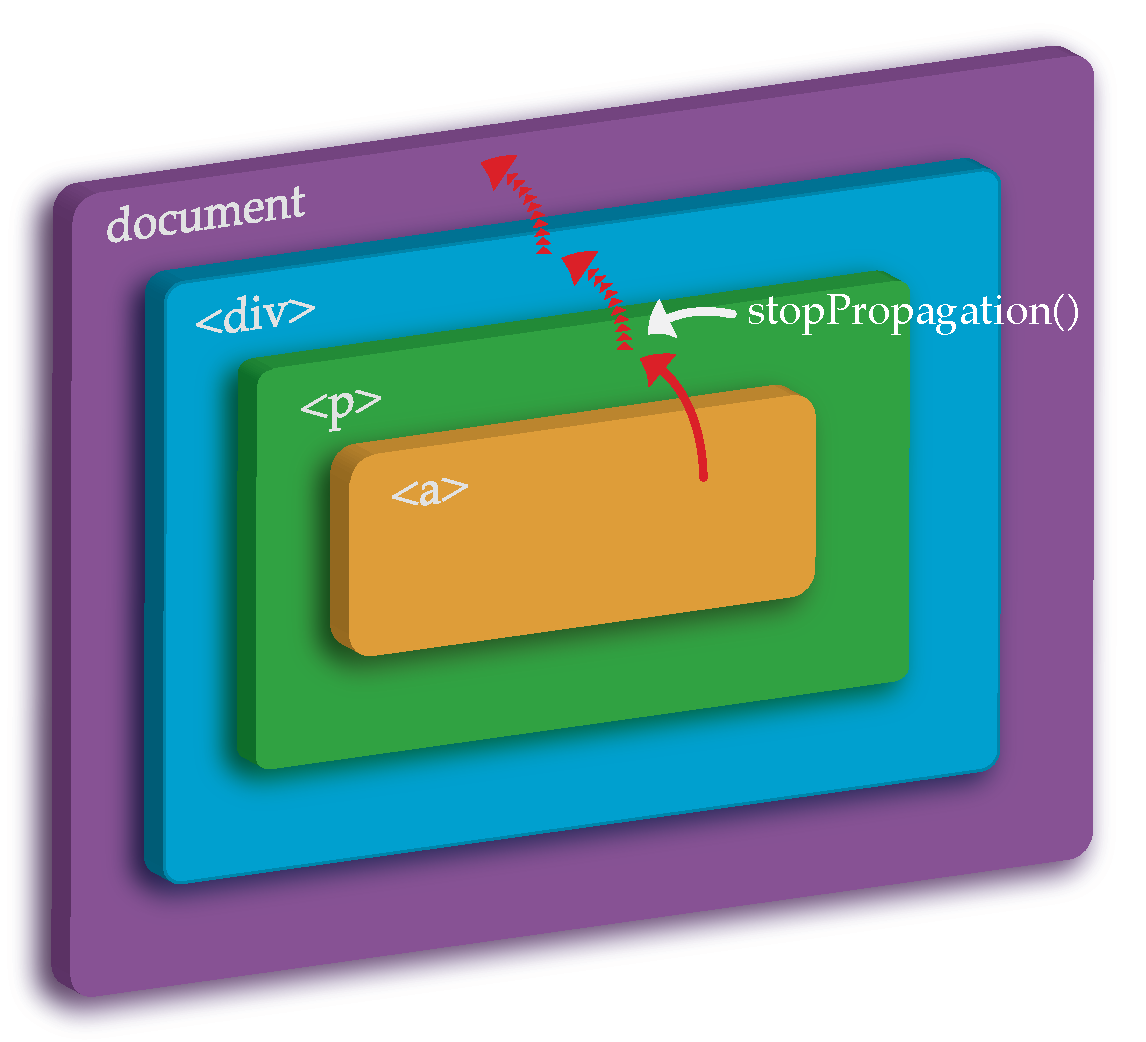
\includegraphics[width=\textwidth]{dom-event-bubbling}
  \caption[DOM event propagation]{DOM event propagation and the effect of stopPropagation()}
  \label{fig:dom-event}
\end{figure}

% subsubsection domobjects (end)

% subsection dom (end)
\subsection{AJAX} % (fold)
\label{sub:ajax}

Since its beginnings, the Web has been document based.
This means that, when the visitor wants more information and clicks on a link, the browser would request and load another whole document.
Even in web applications, the browser would have to reload the full page to send any information from the user and update the page.

\begin{wrapfigure}{r}{0.5\textwidth}
  \centering
    \includegraphics[width=0.48\textwidth]{logo-not-ajax}
  \caption[AJAX logo]{This is not the \idx{AJAX} logo you are looking for}
  \label{fig:ajax-logo}
\end{wrapfigure}

This turns out to be inefficient and overkill in most situations, since web applications do not need to reload the full page in every user interaction but only update a little amount of information.
To address this problem several solutions where developed, from frames to applets, but they were too cumbersome or foreign respect the basic web technologies.

In 1999, \idx{Microsoft} proposed and implemented in its \idx{Internet Explorer} a new \idx{ActiveX} control to asynchronously load new data from the server without need to reload the page.
Using \idx{JavaScript}, that data could be requested on demand once the page was loaded, and through callbacks the data could be processed and the user interface changed accordingly.

Later, the rest of the browsers vendors implemented a similar technology under the \idx{XMLHttpRequest} object.
As this was gradually introduced, web developers started using it but it did not become a popular approach until 2004, when several big web applications such as \idx{Gmail} were developed.

Then, the term \ida{AJAX} was coined \cite{AJAX} to designate the technologies involved in the process, though most of them can be replaced by others while maintaining the same spirit.
Seeing how useful it had become, the \ida{W3C} decided to standardize the \idx{XMLHttpRequest} object.

As depicted in Figure~\ref{fig:ajax-application-model}, this approach needs another layer of complexity in the client to handle the data and update the interface.
This \ida{AJAX} engine means that much more \idx{JavaScript} code in the client is needed.
Eventually, this enables the rise of heavy web applications running in the client, with a substantial codebase to maintain and support across several browsers.

\begin{figure}[htbp]
  \centering
    \includegraphics[width=\textwidth]{ajax-application-model}
  \caption[AJAX web application model]{AJAX web application model compared to the classic one.\newline© Jesse James Garrett}
  \label{fig:ajax-application-model}
\end{figure}

From the point of view of the user, the experience is much less disruptive than the classic model, as seen on Figure~\ref{fig:ajax-flow}.
When a user clicks a link or a button in a traditional web application, the user interface blocks, goes blank, and he has to wait until another page is fully reloaded if he wants to continue with another task.

\begin{figure}[htbp]
  \centering
    \includegraphics[width=\textwidth]{ajax-flow}
    \caption[AJAX flow]{Flow of the actions in a AJAX web application.\newline© Jesse James Garrett}
  \label{fig:ajax-flow}
\end{figure}

In an \idx{AJAX} application, when the user performs such actions, the interface does not block; instead the \idx{AJAX} engine is notified and the interface is \emph{instantly} available.
Meanwhile, backstage data gets interchanged and the client is updated, so that it can refresh the interface using the \ida{DOM} and a mix of \ida{HTML} and \ida{CSS}.

Though it could appear that the application has more overhead now, the user will notice a much more responsive application. Also, the requests should be much faster than before, since the browser does not need to process again all the resources or redraw the whole page, and the server only needs to generate fragments of data.

However, there are some drawbacks to this approach.
The first one is that the browser offers no feedback whatsoever to the user, but that is easily solved: the interface needs to reflect some visual feedback, like a spin ball.
The second one is that the application will break the history of the user, since no new page has been served, it cannot go back to the previous state or even link to it.
This has also been solved by the \ida{HTML}5 History \ida{API}, that allows to manipulate the browser history.

The third and hard one is that users with \idx{JavaScript} disabled will not be able to use this web application at all.
The best practice is to offer an alternate version with plain \ida{HTML} pages, but sometimes that is not possible or it makes no sense.
In the case of this project, since it was mostly experimental and not oriented for mainstream users, it was decided that such alternative would not be developed.

\subsubsection{How XMLHttpRequest works} % (fold)
\label{ssub:xmlhttprequest}

First of all, a \idx{XMLHttpRequest} object must be created, and a custom function that will be act as a callback must be set in its \texttt{onreadystatechange} property.
The next step consists of opening the connection to the server, with its \texttt{open()} method, specifying at least three parameters: first the \ida{HTTP} method to use (\texttt{"GET"} or \texttt{"POST"}), then the url that we wish to contact and finally if the requests should be asynchronous or not.
This last parameter is usually set to \texttt{true}, otherwise the user interface will block.

From now on, this object can make as many requests as it needs.
To make a request its \texttt{send()} method is used, with additional data if the method is \texttt{POST} or with no data (or \texttt{null}) if the method is \texttt{GET}.
Additionally, and only if needed, the \texttt{setRequestHeader()} method could be used to modify the headers of the \ida{HTTP} request.
If the request is asynchronous, the flow of the program will continue normally; if not, the program will block until the server sends all the data.

Some time later, the server will answer with the response data.
Then, the callback specified in the \texttt{onreadystatechange} property will be called, with all the needed data already updated in the \idx{XMLHttpRequest} object.
Actually, this callback will be called not only once but several times, each time reporting the progress of the request.
To be sure that the request was completed it is need to check that the \texttt{readyState} property is exactly 4, and to know that the requested resource is ok that the \texttt{status} property is 200 (this is the \ida{HTTP} state response).

If after that all was according to plan, the plain data will be accessible from the \texttt{reponseText} property.
Also, if the response is in \ida{XML}, the \texttt{reponseXML} property is also available with the parsed \ida{XML} tree (the reason of the X in \ida{AJAX}).
The callback will then usually make some \ida{DOM} manipulation to reflect the change in the interface.

Given the usefulness of this technique, most third-party libraries have implemented wrappers and more straightforward \ida{API}s to cover more use cases.
Also, there are different variations, for example the current trend is not to use the \ida{XML} format but to transmit everything in \ida{JSON}, a much more efficient markup language that is native to \idx{JavaScript}.

% subsubsection xmlhttprequest (end)

\subsubsection{JSONP} % (fold)
\label{ssub:jsonp}

By design, \idx{XMLHttpRequest} carries a severe restriction: it is only allowed to request \ida{URL}s from the same domain.
There are security reasons for this decision, but in this mashup golden era it hinders a lot of its purposes.
Thankfully, another technique has been popularized: \ida{JSONP}.
Less elegant than \ida{AJAX} but equally effective in most situations and without that ugly restriction.

The concept is simple and it is based on the fact that it is possible to add external scripts to a webpage.
Just add a \texttt{script} tag with the desired \ida{URL} and it will be executed; use the \ida{DOM} and that script can be dynamically added after the page is loaded, just like \ida{AJAX}.
Of course, that script must be written in \idx{JavaScript}, so that explains why  \ida{JSON} is used to pass the required data.

Listing~\ref{jsondata} shows how some data could be expressed in \ida{JSON} so that it can be used as an \ida{AJAX} response.
A question appears, how is that data going to be executed in order to access it?
The answer is by telling the external server to wrap it up in some function that we have define in our \idx{JavaScript} code.
The way to tell that to the other server is to add the name of the function to the requested \ida{URL} as a parameter (usually called \texttt{jsonCallback} or just \texttt{callback}).

\begin{lstlisting}[language=JavaScript,label=jsondata,caption=Some JSON data]
  {
    name:   "Kermit",
    animal: "Frog",
    age:    56,
    height: 45
  }
\end{lstlisting}

For example, if we tell the other server that the function is called \texttt{doSomethingWithData()}, it can then wrap it up in a way that the data is the parameter for that function (see Listing~\ref{jsonpdata}).
Since this code will be executed in our web application, it will call that function with that data at the exact moment the file is received and parsed.
Therefore, that function must be defined in the global object, so it can process the received data without any problem.

\begin{lstlisting}[language=JavaScript,label=jsonpdata,caption=Same JSON data wrapped in a custom function]
  doSomethingWithData({
    name:   "Kermit",
    animal: "Frog",
    age:    56,
    height: 45
  });
\end{lstlisting}

Obviously, the server must explicitly support this technique, otherwise it is impossible to receive and change the server response without the use of proxies.
Also, \ida{JSONP} should only be applied with trusted third parties, since any malicious code could be injected in the page.
The last security concern is that \texttt{POST} is not \emph{supported}, so any parameter has to be passed using \texttt{GET}, i.e., adding the parameters to the \ida{URL}.
However, due to its utility, almost all the popular libraries have similar tools that homogenizes  the use of \ida{AJAX} and \ida{JSONP}.

% subsubsection jsonp (end)

% subsection ajax (end)

% section javascript (end)
\section{JavaScript Framework: \idx{MooTools}} % (fold)
\label{sec:mootools}

Before explaining why \idx{MooTools} has been chosen for this application, another important question needs to be resolved.

\subsection{Why Use a \idx{JavaScript} Framework?} % (fold)
\label{sub:whymootools}

There are several reasons that lead to this conclusion, the most important are:

\begin{itemize}

  \item Because we want to support different browsers.
  If we do not use a framework a lot of time would be spent debugging the huge differences between \idx{Internet Explorer} and the rest of the browsers.

  \item Because we want to facilitate the development, since usually these frameworks cover several holes in the \idx{JavaScript} specification that allows us fixing common issues with less code.

  \item Because we want the interface to have advanced effects.
  We could just search for several scripts that makes one individual effect, but that will result in redundancies, differences in quality code and waste time in searching.

\end{itemize}

% subsection whymootools (end)

\subsection{Making the Decision} % (fold)
\label{sub:decision}

By the previous standards, we have plenty of options to choose from:
\idx{jQuery}\footnote{\url{http://jquery.com/}},
\idx{Prototype}\footnote{\url{http://www.prototypejs.org/}},
\idx{Dojo}\footnote{\url{http://www.dojotoolkit.org/}},
\idx{YUI}\footnote{\url{http://developer.yahoo.com/yui/}},
\idx{GWT}\footnote{\url{http://code.google.com/webtoolkit/}},
\idx{Ext JS}\footnote{\url{http://www.extjs.com/}}, etc.
Overall, these are very popular and they offer high quality and plenty of functionality.
However, for this particular project, and after some consideration, \idx{MooTools}\footnote{\url{http://mootools.net}} was considered the best option.
The reasons for this decision are:

\begin{description}

  \item[Compact] It has a low footprint on the site load because it is reasonably lightweight for the functionality it offers.
  Particularly, it is more optimized in this aspect than \idx{Prototype}, \idx{YUI} or \idx{Dojo}, but it is also slightly more compact than \idx{jQuery}.

  \item[Modular-Based] Because of that, the installation can be customized to get only the modules we need, and the creation of our own extensions is easier.

  \item[Compatible] It has been tested with most browsers: \idx{Internet Explorer} 6+, \idx{Firefox} 2+, \idx{Opera} 9+, \idx{Safari} 2+ (and other \idx{Webkit}-based browsers, like \idx{Chrome}).

  \item[Functional] It offers all the functionality required for the first phase of the project: \idx{drag\et drop}, resize, animations, etc.

It also offers other functionality like \idas{AJAX} support, \idc{Hash} handling or \idc{Cookie} handling, that ease the development in different browsers.

  \item[Object-Oriented] By adding \emph{Classes} to \idx{JavaScript}, an abstraction that it is perfect for this application, since the server code is written is \idx{Java}.

This way, we can use similar concepts both in the server and in the client. Moreover, the inherited code for \idx{ScaleNet} already used \idx{JavaScript} objects.

  \item[Extensive] It also has a repository for official plugins called  \idx{MooTools More} (with similar code quality and documentation to the \idx{MooTools Core}) and other third-party plugins can be found in the web.

  \item[Well-documented] It has extensive documentation for every class of the  framework.

  \item[Well-structured] Its structure is perfect for a professional web application.
  Frameworks like \idx{jQuery} are more focused in reducing the  lines of code that in encouraging robust coding.
  \idx{MooTools} also helps reducing the lines of code, but it has more tools for writing code in a very modular, reusable and robust way, for example by using classes and other abstractions.

  It also improves the readability of the code, something hard to do in \idx{JavaScript}.
  Another important point of this framework is that it is based on prototype extensions (mainly \idc{DOM} extensions), so the syntax is very Object-Oriented and the code seems very clean.

  \item[Used by the \ac{APE} server\index{APE server}]
  So if we use that component, it will be very straightforward to write extensions in \idx{JavaScript} also in the server.
  This will mean that we could use the same coding style and the same tools in the server as in the client.

\end{description}

% subsection decision (end)

% section mootools (end)

\section{Push Server: the APE Server} % (fold)
\label{sec:ape}

Because of technical limitations of traditional browsers, it is not trivial to develop real time applications with \idx{JavaScript}.
More precisely, since it cannot directly push data from the server to the browser, the only native solution is to poll in regular time intervals --- an inefficient approach.

The apprehended solution in the old system was to embed a \idx{Java applet} solely to communicate with the server.
The \idx{Java} \ida{API} for applets includes support for sockets, so it is possible to pass data in real time.
However, the big drawback is that it needs the \idx{Java} plugin to be installed in browsers, and there is no plugin for mobile browsers --- neither in \idx{iOS} nor in \idx{Android}.

It was decided that mobile browsers must be supported by the second iteration of this project, so a new solution native to those browsers should be considered, getting rid of this \idx{Java applet}.

\subsection{Comet} % (fold)
\label{sub:comet}

Shortly after \ida{AJAX} was popularized, another technique ---called in contrast \idx{Comet}--- was developed to solve the particular use case of pushing data from the server to the client.
Since then, several alternatives for creating real-time applications have been developed:

\begin{figure}[htbp]
  \centering
    \includegraphics[width=\textwidth]{comet-flow}
  \caption[Comet flow]{Typical flow in a Comet application (compare with Figure~\vref{fig:ajax-flow})\newline© Alex Russell / \url{infrequently.org})}
  \label{fig:comet-flow}
\end{figure}

\begin{description}
  \item[\idx{WebSocket} \ida{API}] An \ida{HTML}5 extension\footnote{\url{http://dev.w3.org/html5/websockets/}} easy to use that just offers a socket to any server.
  This would be the perfect choice (and it should be chosen in the future), but at the moment it severely lacks support among the supported browsers, so it cannot be considered.
  \item[\idx{Socket.IO}] Since real sockets in browsers are out of the equation, an application with both browser and server components is the only way to go.
  One of the options with a brighter future relies on \idx{NodeJS}\footnote{\url{http://nodejs.org/}}, an effort to bring \idx{JavaScript} to the server.
  
  \idx{Socket.IO}\footnote{\url{http://socket.io/}} is a simple software that simulates real sockets in the browsers and uses \idx{NodeJS} for its server component.
  It holds quite interesting ideas, but it was discarded because then it was in a pretty immature state.
  \item[\idx{CometD}] This is a similar approach by the \idx{Dojo} Foundation\footnote{\url{http://cometd.org/}} (so it works well with the dojo framework), creating a new protocol called Bayeux\footnote{\url{http://svn.cometd.com/trunk/bayeux/bayeux.html}}.
  In a quick glance it was rejected because it seems too complex for this task, and it could end in adding an additional framework in the mix.
  \item[\ida{APE} server] And finally we get to the winner of our contest.
  The \ida{APE} project\footnote{\url{http://www.ape-project.org/}} is a solid full solution with two components (server/browser), and it is focused on supporting real time data streaming.
  Just visiting its website explains why it seems like a better solution, because of the extensive documentation and well-explained examples --- from simple to advanced ones.
  
  One of the reasons why it was chosen it that it offers many layers of tinkering.
  If we only want a socket to a existing server, it has a proxy socket built so it is not needed to write any additional server code.
  But if we need to develop an advanced application, custom modules for the server can be written in \idx{JavaScript}.
  
  The other big reason is that it is written with \idx{MooTools}, so bringing \ida{APE} to the table bears little overhead for the client code.
  In the server, a hypothetical custom module could benefit from having the same framework as in the browser.
\end{description}

After considering all options, the \ida{APE} project looked the most promising one.
Eventually, just the proxy socket was needed, so it was merely a drop-in replacement for the \idx{Java applet}.
In any case, as its server deployment (see \S\vref{sec:deployment}) consists on almost exclusively installing the \idx{Debian} \ida{APE} package, it results in an elegant and painless solution.

% subsection comet (end)

\subsection{How the APE Server Works} % (fold)
\label{sub:how_the_ape_server_works}

As we said, the system needs two components: one to be installed in the server and a script to be included in our web application.
The first component is a typical web server that listens upon a port, with the special peculiarity that only understands the \ida{APE} protocol.

\begin{wrapfigure}{r}{0.5\textwidth}
  \centering
    \includegraphics[width=0.48\textwidth]{ape-comic}
  \caption{Real official APE documentation}
  \label{fig:ape-comic}
\end{wrapfigure}

In that server, modules can be written in \idx{JavaScript} (or even \idx{C}), with a convenient \ida{API} to access common web resources like sockets, pipes or \idx{MySQL} connections.
There are some modules and plugins implemented by default, like one that acts as a proxy for \ida{TCP} sockets, or other that redirects data from a server application to the client.
With those two simple modules a lot of applications can be written without needing a custom module.

The server maintains a list of named channels; each channel holds one or more users that can write and read from that channel.
Again, every user can have more than one connection, for example a user that has two tabs open in the same browser, or that have two sessions in two different devices at the same time.
For this, the server \ida{DNS} must be configured to answer to multiple dynamic subdomains  (\verb|1.ape.domain.com|, \verb|2.ape.domain.com|, \verb|42.ape.domain.com|, etc).

In the browser, a set of scripts must be added to our web application so that they can talk with the backend: the \ida{APE} \ida{JSF}.
The configuration is very basic: it only needs the \ida{URL} for the rest of the scripts and the base domain of the \ida{APE} server.

\begin{lstlisting}[language=JavaScript,label=apesocket,caption=TCPSocket usage in APE JSF]
var client = new APE.Client();
var socket;

client.load();
client.addEvent('load', function() {
  this.core.start();
});

client.addEvent('ready', function() {
  socket = new this.core.TCPSocket();
  socket.open(host, port);
  socket.onopen = function() {
    socket.send('hello world');
  };
  socket.onread = function(msg) {
    console.log('New message: ' + msg);
  };
  socket.onclose = function() {
    socket = null;
    console.log('Connection with the server closed.');
  };
}

window.addEvent('unload', function() {
  socket.close();
}
\end{lstlisting}

Then the \ida{APE} client can be created, the connection opens and the two parties start exchanging messages.
Messages are formatted as \ida{JSON} arrays that contains two groups of objects: \emph{commands} and \emph{raws}.
The former ones come from browsers to the server while the latter ones go the other way around.

Commands should be taken as actions that the clients want to accomplish, like opening the connection or sending some data.
Commands are composed by a name, a challenging number (increased each time, to numerate the messages) and optional parameters.
Depending on the name, the message is processed by the very \ida{APE} server or served to a custom module that will answer to that action.

Raws can be expressed as data sent by the server, indeed it is composed by a name, a timestamp and the data as a \ida{JSON} object.
Again, the name reveals the purpose of the transmission and the data format.
It is not uncommon for a message (that is, a \ida{JSON} array) to contain more than one raw.

To send a command, the client creates a \idc{GET} or \idc{POST} request to a increasingly numerated subdomain, encoding the \ida{JSON} array as the only parameter.
When there is data to send, the server answers and the raw(s) can be found in the body response.

% subsection how_the_ape_server_works (end)

\subsection{Transport Methods} % (fold)
\label{sub:transport_methods}

Though it is not completely essential to know how exactly the \ida{APE} server works in the backend, it should be understood how it earns its push capabilities.
There are four transport methods implemented that the developer can choose from, but each of them has its strengths and weaknesses.

\begin{description}
  \item[\idx{Long-polling}] This is the default transport method (so it will be selected unless noted otherwise), and it works in pretty much every \idx{JavaScript}-enabled browser.
  It is based on \ida{AJAX} but with a twist: the client request a resource but the server keeps the \ida{HTTP} connection open until it has something to say.
  
  When there is data to send (or after a certain timeout), the server sends the response.
  Then, the client immediately re-request the same resource, so the server has always a connection open to the browser.
  Of course, the main drawback of this approach is that it is more like a hack, so it could be done more efficiently.
  \item[\ida{JSONP}] Similar to the previous one but over \ida{JSONP} instead of \ida{AJAX}, so it offers cross-domain possibilities.
  \item[\idx{XHRStreaming}] Also very similar to the first one, with the exception that the server do not close the connection when it has information to send.
  Therefore it only needs one connection, so it is more efficient.
  Sadly, this only works with recent browsers.
  \item[\idx{WebSocket}] As said before, this only works in a few new browsers, so it does not make sense to support it just yet if most times it is going to fallback to the default transport method.
\end{description}
% subsection transport_methods (end)
% section ape (end)
\section{Mobile Web Development} % (fold)
\label{sec:mobile}

Web development has been, from the beginning, device independent.
Every device can access the same page and format it differently to a certain screen resolution.
Of course some of the less powerful devices suffered restrictions, since they could not handle \idx{JavaScript}, full \ida{CSS} or even images.

With the rise of touch devices like the \idx{iPhone} or the \idx{Android} phones, it appeared a new wave of mobile browsers capable of render websites almost as exactly as desktop browsers.
The beautiful thing about these new mobile browsers is that they are all based on the \idx{Webkit} engine.

\begin{figure}[htbp]
  \centering
    \includegraphics[width=\textwidth]{iphone-ipad-android}
  \caption[Mobile devices with Webkit]{An iPhone, iPad and Android, the three most popular mobile platforms that run Webkit}
  \label{fig:iphone-ipad-android}
\end{figure}

They can display more or less features, but they are somewhat homogenous in their implementation.
Also, since they are very recent, modern standards like \ida{HTML}5 and \ida{CSS}3 are widely supported.

The most important thing to notice is that the user input is notably different from a traditional computer.
Instead of using a mouse to go to an exact pixel in the screen, the user directly touches the display with his fingers.
This calls for new paradigms, since not all interfaces are cut for this kind of interaction:

\begin{itemize}
  \item Buttons must be bigger, since fingers are not as precise as mouses.
  \item The whole interface need to be at a certain size, since a good mobile web application should not require the user to zoom to see the content.
  This usually means less information in the screen.
  \item More than one finger can be used, in contrast to only one mouse in the desktop.
  That enables several new gestures, like pinching, that are newly available to web applications.
  \item By default, drag\et{}drop is reserved to scroll the page.
  If the web application needs to use it, like the current web interface does, it has to capture all finger events and re-create the scrolling experience.
  \item Double tapping is a movement that makes more sense on these devices than in desktop web applications, and it could be seen as a right click gesture on the desktop.
  \item There is also very important to notice that the screen could be oriented in portrait or landscape, so the interface must be adaptable.
\end{itemize}

The current \idx{ScaleNet} interface, being optimized for big screens, it is not even usable on these devices.
Even when zooming manually, most actions rely on drag\et{}drop and therefore are not even accessible, so it is impossible to move or delete a session.
It is clear that if these devices have to be supported, a mobile version needs to be developed fixing those issues.

To deal with these peculiarities, there are several additions to the web stack tools to make nicer web applications.
This applies specially in \idx{iOS} devices, but \idx{Android} also understands some of them.
The most useful and distinct features are:

\begin{description}
  \item[Touch events] Since mouse events do not make any sense there, special custom events for \emph{touches} and gestures are available.
  \item[Viewport] To deal with the fact that most websites are developed for bigger screens, by default web applications are rendered against a virtual viewport wider than the real screen.
  Then, it is up to the user to zoom in to read the page.
  
  At the same time, web applications specially designed for these devices can detect them and define the size of the viewport, so the user do not have to zoom to have a decent experience.
  Another solution is the use of \idx{CSS}3 conditional styles and media queries.
  \item[Special forms] While maintaining most of the form elements, there are some missing ---like file uploading--- and some new interface elements ---like select boxes.
  There are extra features that can be triggered like autocompletion, autocorrection, autocapitalize, custom keyboards for numbers/emails, etc.
  Moreover, since the virtual keyboard could appear, web applications should be prepared for having very little room.
  \item[App icon] Both \idx{iOS} and \idx{Android} allow the creation of shortcuts to display in the home screens.
  For that, it is possible to define the icons that those shortcuts can use.
  \item[Hiding the browser \ida{UI}] Once a web application is launched from an \idx{iOS} shortcut, it can dictate if the browser \ida{UI} should be hidden or not.
  In the case that the \ida{UI} is hidden, it can also define which aspect should the menubar have (light, dark or transparent).
  \item[Startup image] Native \idx{iOS} apps can specify a startup image to be displayed when loading the application.
  More than being a visual triviality, it is designed to display an empty interface so that the user \emph{feels} that the application loads faster.
  Web applications can also set such an image with a meta tag.
\end{description}

\begin{wrapfigure}{r}{0.5\textwidth}
  \centering
    \includegraphics[width=0.48\textwidth]{iscroll}
  \caption{iScroll in action}
  \label{fig:iscroll}
\end{wrapfigure}

Lastly, it has to be noted that there are mobile \idx{JavaScript} frameworks that have been developed with these restrictions in mind.
Some of them try to bring a lightweight framework like \idx{Zepto.js}, others try to develop a full solution for web applications like \idx{Sencha} or \idx{JQTouch}, and others just try to ease the development of specific features.

For this project, one of those frameworks was used: \idx{iScroll}\footnote{\url{http://cubiq.org/iscroll}}.
The goal of this script is to provide a scrolling effect inside an element, since the only scrolling available in these mobile browsers is the page scrolling.
With mostly three lines of setup, this script simulates that native scrolling effect with some advanced \ida{CSS}3 properties (animations and so on).

The common use case for this effect is the implementation of a bottom toolbar, like in native apps.
These mobile browsers do not offer support for fixed positioned elements, so this is the only way that this kind of toolbar can be simulated.

% section mobile (end)

\chapter{Development} % (fold)
\label{cha:development}

\setlength{\epigraphwidth}{10cm}
\renewcommand{\tabcolsep}{0em}

\epigraph{
  \begin{tabular}{p{1.75cm}p{8cm}}
    \footnotesize{\textbf{\textsc{Walter}} :}
      & Did you learn nothing from my chemistry class? \\
    \footnotesize{\textbf{\textsc{Jesse}} :}
      & No. You flunked me, remember? You prick! Now let me tell you something else. This ain't chemistry ---this is art. Cooking is art. And the shit I cook is the bomb, so don't be telling me. \\
    \footnotesize{\textbf{\textsc{Walter}} :}
      & The shit you cook is shit. I saw your set-up. Ridiculous. You and I will not make garbage. We will produce a chemically pure and stable product that performs as advertised. No adulterants. No baby formula. No chili powder. \\
    \footnotesize{\textbf{\textsc{Jesse}} :}
      & No, no, chili P is my signature! \\
    \footnotesize{\textbf{\textsc{Walter}} :}
      & Not anymore. \\
  \end{tabular}
  \vspace{1em}
}{\textit{Pilot}\\ \textsc{Breaking Bad}}

\newpage

\section{Introduction} % (fold)
\label{sec:intro3}

Last chapter was focused in work done by others; this chapter brings light to the actual work done in this project, a new iteration on the \ida{PNAI}.
As the previous compilations were needed to understand the environment of this work, the following sections explain which additions were requested and developed.

User requirements are the first thing to clarify, extracted from the received from tutors and other \ida{T-Labs} members previously involved in the project.
This feedback was continually given as the project evolved, mostly for design concerns or when adding additional technologies, not for the implementation itself.

Later on, the system design is elucidated with diagrams that highlight the changes respect the base version, detailing the implementation process.
Furthermore, noteworthy hiccups found in the implementation process are specified using the resulting algorithms and solutions.

% section intro3 (end)

\nicesectionending
\section{New Requirements} % (fold)
\label{sec:new_requirements}

There are new requirements that need to be satisfied within the redesigned \ida{PNAI} interface.
These requirements were extracted in several team meetings as the work advanced.
They could be divided into roughly three phases: a initial phase (a full redesign), a second phase (adding more functionality) and a third phase (implementing the mobile version).

\subsection{User Requirements} % (fold)
\label{sub:user_requirements}

As this was a new iteration over an already developed product, there were multiple requirements that were already set and implemented.
Those requirements are not discussed since they are out of the limits of this work.
Therefore, this is a list of only the new requirements resulted from the team feedback:

\begin{center}
  \begin{userrequirement}[Redesign interface]
    \label{tab:requirementredesign}%
    \requirementprio{High}
    \requirementphase{Initial phase}
    \requirementdesc{Overall design must be modernized, keeping the same elements, but giving a fresher, more professional look.
    Animations could be included to give a more responsive experience.}
  \end{userrequirement}
\end{center}

\begin{center}
  \begin{userrequirement}[Adapt to different resolutions]
    \label{tab:requirementreadapt}%
    \requirementprio{High}
    \requirementphase{Initial phase}
    \requirementdesc{The new design must not be static like the previous one, it must adapt when the user resizes the browser so that it fills in the available space and does not trigger browser scrollbars.}
  \end{userrequirement}
\end{center}

\begin{center}
  \begin{userrequirement}[Show device name]
    \label{tab:requirementdevicename}%
    \requirementprio{Medium}
    \requirementphase{Initial phase}
    \requirementdesc{The device name (set by the user) must be displayed besides the device representation.}
  \end{userrequirement}
\end{center}

\begin{center}
  \begin{userrequirement}[Load real user devices]
    \label{tab:requirementrealdevices}%
    \requirementprio{Low}
    \requirementphase{Initial phase}
    \requirementdesc{The old interface always loaded the same three devices, independently of the user and its real registered devices.
    This new interface shall support an undefined number of devices, and load them dynamically at the beginning.
    It also shall create or delete devices at any moment when the backend commands it.}
  \end{userrequirement}
\end{center}

\begin{center}
  \begin{userrequirement}[Put screenshots in session icons]
    \label{tab:requirementscreenshots}%
    \requirementprio{Low}
    \requirementphase{Initial phase}
    \requirementdesc{The old interface always showed the same generic icon for all sessions.
    This new interface shall show the real screenshot already stored for each video file.}
  \end{userrequirement}
\end{center}

\begin{center}
  \begin{userrequirement}[Reorganize devices]
    \label{tab:requirementreorganize}%
    \requirementprio{Medium}
    \requirementphase{Initial phase}
    \requirementdesc{User must be able to move around its devices in the \ida{PNAI} interface, reordering them as they wish.
    In any case, all devices must be fully visible at any time.}
  \end{userrequirement}
\end{center}

\begin{center}
  \begin{userrequirement}[Resize devices]
    \label{tab:requirementresize}%
    \requirementprio{Low}
    \requirementphase{Initial phase}
    \requirementdesc{User must be able to scale its devices in the \ida{PNAI} interface, making them bigger or smaller, within certain bounds to guaranty that sessions have room to be drawn inside them.}
  \end{userrequirement}
\end{center}

\begin{center}
  \begin{userrequirement}[Browser compatibility]
    \label{tab:requirementcompatible}%
    \requirementprio{High}
    \requirementphase{Initial phase}
    \requirementdesc{It shall be compatible with latest versions of all popular devices: \idx{Internet Explorer} 7+, \idx{Firefox}, Opera, Safari and Chrome.
    The only exception shall be \idx{Internet Explorer} 6, for practical reasons.}
  \end{userrequirement}
\end{center}

\begin{center}
  \begin{userrequirement}[Integrate the \idx{IPTVplus} interface]
    \label{tab:requirementiptv}%
    \requirementprio{High}
    \requirementphase{Second phase}
    \requirementdesc{The \idx{IPTVplus} interface (see Figure~\ref{fig:iptvplus}) must be implemented as a sidebar inside the \ida{PNAI} interface.
    That way, the user must be able to buy new content within the \ida{PNAI} interface, all just in one page.}
  \end{userrequirement}
\end{center}

\begin{center}
  \begin{userrequirement}[Buy content onto a device]
    \label{tab:requirementcontentdevice}%
    \requirementprio{Medium}
    \requirementphase{Second phase}
    \requirementdesc{When the user buys new content from this \ida{PNAI} interface, it shall be able to select another device as the destination to directly play that content other than the default device.}
  \end{userrequirement}
\end{center}

\begin{center}
  \begin{userrequirement}[Buy content onto a buddy]
    \label{tab:requirementcontentbuddy}%
    \requirementprio{Medium}
    \requirementphase{Second phase}
    \requirementdesc{When the user buys new content from this \ida{PNAI} interface, it shall be able to select another buddy as the destination to directly play that content.}
  \end{userrequirement}
\end{center}

\begin{center}
  \begin{userrequirement}[Resize/collapse sidebar]
    \label{tab:requirementsidebar}%
    \requirementprio{Medium}
    \requirementphase{Second phase}
    \requirementdesc{The user must be able to horizontally resize the sidebar to a custom size, that must be less than 50\% of the page width.
    Therefore, the \idx{IPTVplus} interface (see Figure~\ref{fig:iptvplus}) must be implemented as a sidebar inside the \ida{PNAI} interface.}
  \end{userrequirement}
\end{center}

\begin{center}
  \begin{userrequirement}[Design and adapt a mobile interface]
    \label{tab:requirementmobile}%
    \requirementprio{High}
    \requirementphase{Third phase}
    \requirementdesc{A new mobile interface must be created for popular modern smartphones with a touchscreen, specifically for the \idx{iOS} and \idx{Android} platforms.
    The interface shall retain all functionality of the \ida{PNAI} desktop interface.
    Elements and abstractions must be adapted to mobile peculiarities so that the user experience is comfortable.}
  \end{userrequirement}
\end{center}

Outside of these requirements, there were some \emph{implied} requirements, due to the experimental nature of this project: this effort was planned for showcasing purposes rather than for real customers.
For example, delivering a product with certain quality but as fast as possible derives on some decisions like trying to not rewrite other parts of the system unless completely necessary.

% subsection user_requirements (end)

\subsection{Software Requirements} % (fold)
\label{sub:software_requirements}

After some deliberation, those previous user-centered requirements result in several software requirements.
These requirements are more specific and precise, giving a more approximate measure of the complexity of the tasks.

\begin{center}
  \begin{softwarerequirement}[Replace the \idx{Java} applet]
    \label{tab:requirementapplet}%
    \requirementprio{High}
    \requirementphase{Third phase}
    \requirementdesc{Both \idx{iOS} and \idx{Android} do not recognize the \idx{Java} applet, so it must be replace with a native \idx{JavaScript} solution.
    This means that all the \idx{Java} code directly related to the applet must be ported to \idx{JavaScript}, and an alternative for pushing data to the browser must be considered.}
  \end{softwarerequirement}
\end{center}

% subsection software_requirements (end)

\subsubsection{Use Cases} % (fold)
\label{ssub:usecasesold}

In the following tables the current supported use cases are explained step by step.
The first use case is detailed in Table~\ref{tab:usecasestopdevice}, explaining the situation where the user wants to stop/delete the session in a device.

\begin{center}
  \begin{usecase}[Stop a session of a device]
    \label{tab:usecasestopdevice}%
    \usecaseactor{System user}
    \usecasepre{A session is already running on a device, and it is showing in the \ida{PNAI} interface inside of that device.}
    \usecasepost{Session must terminate, i.e., the content must stop playing. The user must be notified with a popup and the session icon must be deleted from the \ida{PNAI} interface.}
    \usecasemain{
      \begin{usecasepath}
        \item User starts dragging the session icon.
        \item A copy of the session icon appears under the user's cursor, and follows the cursor until the user drops it.
        \item User drops the cloned session icon into the trash.
        \item A popup appears to notify the user that the action is in progress and the cloned session icon is deleted from the view.
        \item The content stops playing.
        \item The popup disappears and the original session icon is deleted from the view.
      \end{usecasepath}
    }
    \usecasealt{1}{
      \begin{usecasepath}[b]
        \setcounter{enumi}{2}
        \item User drops the session into a blank space.
        \item Action is cancelled.
      \end{usecasepath}
    }
    \usecasealt{2}{
      \begin{usecasepath}[c]
        \setcounter{enumi}{4}
        \item There is an error with the server and the content keeps playing.
        \item The content of the popup changes to notify the user that there was an error with the server and the action could not be completed.
        After 5 seconds it disappears.
        \item Action is cancelled.
      \end{usecasepath}
    }
  \end{usecase}
\end{center}

\begin{figure}[htbp]
  \centering
    \includegraphics[width=\textwidth]{pnai-old-stop}
  \caption{Deleting a session in the old \idx{PNAI}}
  \label{fig:pnai-old-stop}
\end{figure}

Figure~\ref{fig:pnai-old-stop} shows how the page looks when it is waiting for a response to the server for the previous use case.
Since the user interface does not block in the process, the communication between the front end and the back end must be asynchronous.
The use case for terminating a session that a buddy is playing and that we own is very similar, as Table~\ref{tab:usecasestopbuddy} exposes.

\begin{center}
  \begin{usecase}[Stop a session of a buddy]
    \label{tab:usecasestopbuddy}%
    \usecaseactor{System user}
    \usecasepre{A session owned by the user is running on a device, and it is showing in the \ida{PNAI} interface near that buddy's name.}
    \usecasepost{Session must terminate, i.e., the content must stop playing. The user must be notified with a popup and the session icon must be deleted from the \ida{PNAI} interface. The buddy is \emph{not} notified, the content stops without warning.}
    \usecasemain{
      \begin{usecasepath}
        \item User starts dragging the session icon.
        \item A copy of the session icon appears under the user's cursor, and follows the cursor until the user drops it.
        \item User drops the cloned session icon into the trash.
        \item A popup appears to notify the user that the action is in progress and the cloned session icon is deleted from the view.
        \item The content stops playing.
        \item The popup disappears and the original session icon is deleted from the view.
      \end{usecasepath}
    }
    \usecasealt{1}{
      \begin{usecasepath}[b]
        \setcounter{enumi}{2}
        \item User drops the session into a blank space.
        \item Action is cancelled.
      \end{usecasepath}
    }
    \usecasealt{2}{
      \begin{usecasepath}[c]
        \setcounter{enumi}{4}
        \item There is an error with the server and the content keeps playing.
        \item The content of the popup changes to notify the user that there was an error with the server and the action could not be completed.
        After 5 seconds it disappears.
        \item Action is cancelled.
      \end{usecasepath}
    }
  \end{usecase}
\end{center}

Tables~\ref{tab:usecasecopydevice},~\ref{tab:usecasecopybuddy},~\ref{tab:usecasetransferdevice}~and~\ref{tab:usecasetransferbuddy} show how the user could copy or transfer a session to another device or buddy.

\begin{center}
  \begin{usecase}[Copy a session to a device]
    \label{tab:usecasecopydevice}%
    \usecaseactor{System user}
    \usecasepre{A session is already running on a device/buddy, and it is showing in the \ida{PNAI} interface inside of that device/buddy. Also, there is another device online.}
    \usecasepost{Session must be copied to that device, i.e., the content must be duplicated and played on that device. The user must be notified with a popup and the session icon must appear in the \ida{PNAI} interface for the second device.}
    \usecasemain{
      \begin{usecasepath}
        \item User starts dragging the session icon.
        \item A copy of the session icon appears under the user's cursor, and follows the cursor until the user drops it.
        \item User drops the cloned session icon into another device that is online.
        \item A popup menu appears where the user dropped the session, giving options to copy/duplicate the session, transfer the session or cancel the action.
        \item The user clicks on the copy/duplicate option.
        \item The popup menu disappears.
        \item A popup appears to notify the user that the action is in progress and the cloned session icon is deleted from the view.
        \item The content starts playing on the destination device.
        \item The popup disappears and the same session icon appears inside of the destination device.
      \end{usecasepath}
    }
    \usecasealt{1}{
      \begin{usecasepath}[b]
        \setcounter{enumi}{2}
        \item User drops the session into a blank space.
        \item Action is cancelled.
      \end{usecasepath}
    }
    \usecasealt{2}{
      \begin{usecasepath}[c]
        \setcounter{enumi}{4}
        \item The user clicks on the cancel option.
        \item Popup menu disappears and action is cancelled.
      \end{usecasepath}
    }
    \usecasealt{3}{
      \begin{usecasepath}[d]
        \setcounter{enumi}{7}
        \item There is an error with the server and the content is not duplicated.
        \item The content of the popup changes to notify the user that there was an error with the server and the action could not be completed.
        After 5 seconds it disappears.
        \item Action is cancelled.
      \end{usecasepath}
    }
  \end{usecase}
\end{center}

\begin{center}
  \begin{usecase}[Copy a session to a buddy]
    \label{tab:usecasecopybuddy}%
    \usecaseactor{System user}
    \usecasepre{A session is already running on a device/buddy, and it is showing in the \ida{PNAI} interface inside of that device/buddy. Also, there is another buddy online.}
    \usecasepost{Session must be copied to that buddy, i.e., the content must be duplicated and played on the buddy's default device. The user must be notified with a popup and the session icon must appear in the \ida{PNAI} interface near the name of that buddy. The buddy is \emph{not} notified, the content plays without warning.}
    \usecasemain{
      \begin{usecasepath}
        \item User starts dragging the session icon.
        \item A copy of the session icon appears under the user's cursor, and follows the cursor until the user drops it.
        \item User drops the cloned session icon into another buddy that is online.
        \item A popup menu appears where the user dropped the session, giving options to copy/duplicate the session, transfer the session or cancel the action.
        \item The user clicks on the copy/duplicate option.
        \item The popup menu disappears.
        \item A popup appears to notify the user that the action is in progress and the cloned session icon is deleted from the view.
        \item The content starts playing on the buddy's default device.
        \item The popup disappears and the same session icon appears inside of the destination buddy.
      \end{usecasepath}
    }
    \usecasealt{1}{
      \begin{usecasepath}[b]
        \setcounter{enumi}{2}
        \item User drops the session into a blank space.
        \item Action is cancelled.
      \end{usecasepath}
    }
    \usecasealt{2}{
      \begin{usecasepath}[c]
        \setcounter{enumi}{4}
        \item The user clicks on the cancel option.
        \item Popup menu disappears and action is cancelled.
      \end{usecasepath}
    }
    \usecasealt{3}{
      \begin{usecasepath}[d]
        \setcounter{enumi}{7}
        \item There is an error with the server and the content is not duplicated.
        \item The content of the popup changes to notify the user that there was an error with the server and the action could not be completed.
        After 5 seconds it disappears.
        \item Action is cancelled.
      \end{usecasepath}
    }
  \end{usecase}
\end{center}

\begin{center}
  \begin{usecase}[Transfer a session to a device]
    \label{tab:usecasetransferdevice}%
    \usecaseactor{System user}
    \usecasepre{A session is already running on a device/buddy, and it is showing in the \ida{PNAI} interface inside of that device/buddy. Also, there is another device online.}
    \usecasepost{Session must be transferred to that device, i.e., playback must be stopped at the source and started at the destination device. The user must be notified with a popup and the session icon must appear in the \ida{PNAI} interface for the second device.}
    \usecasemain{
      \begin{usecasepath}
        \item User starts dragging the session icon.
        \item A copy of the session icon appears under the user's cursor, and follows the cursor until the user drops it.
        \item User drops the cloned session icon into another device that is online.
        \item A popup menu appears where the user dropped the session, giving options to copy the session, transfer/hand over the session or cancel the action.
        \item The user clicks on the transfer/hand over option.
        \item The popup menu disappears.
        \item A popup appears to notify the user that the action is in progress and the cloned session icon is deleted from the view.
        \item The content stops playing on the source device.
        \item The content starts playing on the destination device.
        \item The popup disappears, the session icon is deleted from the view and created again inside of the destination device.
      \end{usecasepath}
    }
    \usecasealt{1}{
      \begin{usecasepath}[b]
        \setcounter{enumi}{2}
        \item User drops the session into a blank space.
        \item Action is cancelled.
      \end{usecasepath}
    }
    \usecasealt{2}{
      \begin{usecasepath}[c]
        \setcounter{enumi}{4}
        \item The user clicks on the cancel option.
        \item Popup menu disappears and action is cancelled.
      \end{usecasepath}
    }
    \usecasealt{3}{
      \begin{usecasepath}[d]
        \setcounter{enumi}{7}
        \item There is an error with the server and the content is not transferred.
        \item The content of the popup changes to notify the user that there was an error with the server and the action could not be completed.
        After 5 seconds it disappears.
        \item Action is cancelled.
      \end{usecasepath}
    }
  \end{usecase}
\end{center}

\begin{center}
  \begin{usecase}[Transfer a session to a buddy]
    \label{tab:usecasetransferbuddy}%
    \usecaseactor{System user}
    \usecasepre{A session is already running on a device/buddy, and it is showing in the \ida{PNAI} interface inside of that device/buddy. Also, there is another buddy online.}
    \usecasepost{Session must be transferred to that buddy, i.e., playback must be stopped at the source and started at the buddy's default device. The user must be notified with a popup and the session icon must appear in the \ida{PNAI} interface near the name of that buddy. The buddy is \emph{not} notified, the content plays without warning.}
    \usecasemain{
      \begin{usecasepath}
        \item User starts dragging the session icon.
        \item A copy of the session icon appears under the user's cursor, and follows the cursor until the user drops it.
        \item User drops the cloned session icon into another buddy that is online.
        \item A popup menu appears where the user dropped the session, giving options to copy the session, transfer/hand over the session or cancel the action.
        \item The user clicks on the transfer/hand over option.
        \item The popup menu disappears.
        \item A popup appears to notify the user that the action is in progress and the cloned session icon is deleted from the view.
        \item The content stops playing on the source device.
        \item The content starts playing on the buddy's default device.
        \item The popup disappears, the session icon is deleted from the view and created again inside of the destination buddy.
      \end{usecasepath}
    }
    \usecasealt{1}{
      \begin{usecasepath}[b]
        \setcounter{enumi}{2}
        \item User drops the session into a blank space.
        \item Action is cancelled.
      \end{usecasepath}
    }
    \usecasealt{2}{
      \begin{usecasepath}[c]
        \setcounter{enumi}{4}
        \item The user clicks on the cancel option.
        \item Popup menu disappears and action is cancelled.
      \end{usecasepath}
    }
    \usecasealt{3}{
      \begin{usecasepath}[d]
        \setcounter{enumi}{7}
        \item There is an error with the server and the content is not transferred.
        \item The content of the popup changes to notify the user that there was an error with the server and the action could not be completed.
        After 5 seconds it disappears.
        \item Action is cancelled.
      \end{usecasepath}
    }
  \end{usecase}
\end{center}

\begin{figure}[htbp]
  \centering
    \includegraphics[width=\textwidth]{pnai-old-duplicate}
  \caption{Duplicating a session in the old \idx{PNAI}}
  \label{fig:pnai-old-duplicate}
\end{figure}

Figure~\ref{fig:pnai-old-duplicate} shows how the popup menu is displayed to the user.
It is a very simple menu with only three links, each of which correspond to an action.

% subsubsection usecasesold (end)

% section new_requirements (end)
\nicesectionending
\section{How the Devices Are Placed}
\label{sec:positioning}

The first time that the user visits the page in a new browser, the system has
to place the devices in the screen. Since the number and type of devices are
different for each user, an algorithm must be used to placed the devices in
the available space.

\subsection{Simplified Algorithm}

The restrictions that we have to comply are:

\begin{itemize}
  \item We have an undetermined number of elements to place.
  \item For the sake of simplicity, the elements and the canvas are
  rectangular.
  \item Every element, including the canvas, has a different size.
  \item We have to place them in the most comfortable way possible, ideally
  using all the space we have.
\end{itemize}

The solution to the above problem is known as a variant of 2-D rectangle
packing and it is, regrettably, NP-hard. At this point, it is clear that we
need a simplification. Furthermore, the original problem also presents a big
issue, as it does not address an important constraint: the possibility of
resizing the elements to fit the canvas.

A simplified algorithm is proposed and implemented, relaxing some terms while obtaining acceptable results. The important concepts are:

\begin{itemize}
  \item The main goal is to draw a virtual grid of M$\times$N cells (like a table). Every cell can be a position for a device.
  \item Indeed, we are going to calculate the smallest grid of M$\times$N cells in which the devices can be placed.
  \item Finally, we are going to resize the elements to fit within that cell, giving that every cell has the same size.
\end{itemize}

To obtain the squared grid for N elements, we simply have to calculate the ceiling of the squared root of N as seen in \eqref{gridx}.

\begin{equation}
  Grid_{x} = \lceil\sqrt{N}\rceil \label{gridx}
\end{equation}

This formula synthesizes the idea that, given a certain number of elements N:

\begin{itemize}
  \item If N is a square number (that is, it exists an integer $x$ that
  fulfills $x^2 = N$), then you could fit a whole grid of $x\times{}x$ with
  N elements.
  \item Otherwise, this integer N must be between the square of two
  consecutive integers, that we are going to call $x$ and $x+1$. That is,
  $x^2 < N$ and $(x+1)^2 > N$. In visual words, that means that a grid of
  size $x$ cannot hold that number of elements, and a grid of size $x+1$ can
  hold that number of elements but there will be empty \emph{cells}.
  \item In that case, we choose the grid of size $x+1$, this way we want to
  apply the ceiling function to the squared root to obtain the next following
  integer.
\end{itemize}

In the following figures we can appreciate what all of this means with real examples, using different number of elements.

(insert images with the disposition of different number of elements in the
grid)

If we look at the examples below, we can guess an improvement without making
the calculation severely complicate. We can see that, at certain points, a
whole row of the grid is completely empty, so we are wasting vertical space.
In theory, we could detect when this happens and try to reduce the vertical
height of the grid by one, effectively converting this squared grid into a
rectangle grid with different number of columns and rows.

Parting from an example: if we have $N = 19$, then we obtain $x = 5$ by
applying the previous formula. This will lead us to a 5x5 grid, but the last
row will be completely empty. The question that we have to ask ourselves is:
how big has to be the rectangle grid in order to be able to place this number
of elements? Briefly, the answer is $x \cdot (x - 1)$. That is a mathematical
way of describing that we are decreasing the number of rows by one. In this
case, we need a grid of $5 \times 4$ elements: that will hold up to 20
elements.

To discover whether we have to decrease the number of columns or not, we must
compare that number $(x \cdot x - 1)$ with the actual count of elements. If we
know that this number is bigger or equals to the number of elements, then we
know that a grid of $x \cdot (x - 1)$ elements can hold those elements. On the
contrary, if we know that this number is strictly lower than the number of
elements, then we know that a grid of $x \cdot x$ is unavoidable. This can be
formulated this way:

\begin{equation}
  Grid_{y} = 
  \begin{cases}
    Grid_{x} - 1 & \text{if } N \leq Grid_{x} \cdot (Grid_{x} - 1),\\
    Grid_{x} & \text{if } N > Grid_{x} \cdot (Grid_{x} - 1).
  \end{cases} \label{gridy}
\end{equation}

Another question appears: Do we need to shrink the grid only by one?
Is there any case in which we have to shrink the grid by two or more?

The answer is no.

We can prove why not by calculating if a grid of $(x - 1) \cdot (x - 1)$
elements can hold more elements that the grid of $x \cdot (x - 2)$.
If that is the case, then we would not need to shrink the grid in any case by
two because the grid will be already horizontally shorter.
It is quick to prove this is true following the steps explained from
\eqref{xdem1} to \eqref{xdem3}.

\begin{eqnarray}
  (x-1) \cdot (x-1) &<& x \cdot (x-1) \label{xdem1} \\
  x^2-2x+1 &<& x^2-2x \label{xdem2} \\
  1 &<& 0 \label{xdem3}
\end{eqnarray}

Then, using this final algorithm, the previous examples will change:

(insert images with the disposition of different number of elements in the grid using the final algorithm)

Using this algorithm we can calculate the height, width, vertical and
horizontal offset for every element. If we want to work with percentages, we
only have to divide the size of the container between the number of columns
and rows. For example, if we want to fill the container at 100\%, then every
element will be of size $100/x \times 100/y$. The actual values
for the offset needed for every particular element is then easy to calculate
if we fill the canvas one by one.

\subsection{Storage Positioning}

Next time an user visits this page, the system will remember the last position
of those elements instead of calculating the grid again. Because the user can
change the size of the window at any time, we cannot relay on fixed
positioning with pixels, because our canvas could be bigger or, worse, smaller
than the one we have calculated. Besides being not very elegant, we can find
several situations where the page is unusable.

The best way to avoid all that trouble is treating every position or size in
terms of percentages. This is how is done in the code, and it allows the user
to resize the window at any time: the devices will be resized dinamically
according to that window size.

To store and retrieve painlessly these values, we are going to take advantage
of an useful \idx{MooTools} class: \idc{Hash.Cookie} \cite{MooHashCookie}.
With this utility, we only have to specify the name for the \idc{Cookie} and
we can store a \idc{Hash} into a \idc{Cookie} without worrying about the
\idc{Cookie} itself.
Besides loading the data of the \idc{Cookie} directly on the \idc{Hash} at its
creation, if we change a value of the \idc{Hash} it will be automatically
updated in the \idc{Cookie}.

The reason for using a \idc{Cookie} is mostly because it reduces complexity on
the server, since it does not have to store the position of every device.
Other good reason is that it is the most simple way of allowing different
arrangements in different places; for example the user may want to arrange
radically different its devices in a big screen like in a TV or on a smaller
screen like in a netbook. Finally, it is universal as it is supported by
almost every browser.

The final decision is to have one \idc{Cookie} for each device.
This is very straightforward for the implementation, since a \idc{Cookie} can
have the name of the container.
Each \idc{Hash} that is stored in every \idc{Cookie} is composed by the four
values needed for positioning the element: \idc{offsetX}, \idc{offsetY},
\idc{width} and \idc{height}.
These values are percentages respect the container (the devices list) and an
\idc{Hash} example is presented in Listing~\ref{cookiehash}.

\begin{lstlisting}[language=JavaScript,label=cookiehash,
  caption=Cookie Hash example]
{
  offsetX: 15,
  offsetY: 50,
  height: 10,
  width: 20
}
\end{lstlisting}

Then, each time the object size or dimension changes, the \idc{Hash} (and
therefore the \idc{Cookie}) is updated. These changes happen mostly in two
situations: when we resize a device (changing its size but no its position) or
when we move around a device (changing its position but not its size).

\nicesectionending
\section{APE Server\index{APE server} Installation and Configuration} % (fold)
\label{sec:apeconfig}

In this section the installation and configuration of the \ac{APE} server\index{APE server} are defined step by step.

\subsection{Install the Server} % (fold)
\label{sub:apeinstall}

The \ac{APE} download page \cite{ApeDownload} contains packages for different operating systems and architectures.
In this case, since the system is Debian-based we should use the DEB package.
Once the correct package is downloaded, it can be installed on the \idx{Application Server} by typing Listing~\vref{apeinstallation} from the same directory as the package is stored.

\begin{lstlisting}[label=apeinstallation,caption=APE installation command]
sudo dpkg -i ape-1.0.i386.deb
\end{lstlisting}

After that, the \ac{APE} server daemon (\idc{aped}) is automatically started with the default configuration \cite{ApeSetup}.
It can be checked by visiting the url \url{webportal.imusu.mobile.dtrd.de:6969}.

\nicesubsectionending

% subsection apeinstall (end)

\subsection{Configure BIND} % (fold)
\label{sub:bind}

The \ida{IMS} core is the machine that provides the \idas{DNS} service through \idas{BIND}, and that service needs to be configured to allow the \ac{APE} server\index{APE server} to use a lot of different dynamic subdomains like \verb|1.ape.webportal|, \verb|2.ape.webportal|, \verb|567.ape.webportal|, etc.

This is how the \ac{APE} server\index{APE server} works by default, and it appears that there is no way to configure the \ac{APE} server\index{APE server} for using only one domain \cite{ApeConfig}.

So, in the file \verb|/etc/bind/imusu.dnszone| located in the \ida{IMS} core
we have to look for the \emph{webportal} entry and change that section to look
like Listing~\vref{bindconf}.

\begin{lstlisting}[label=bindconf,caption=BIND configuration]
webportal               1D IN A         192.168.5.234
ape.webportal           1D IN A         192.168.5.234
*.ape.webportal         1D IN CNAME     ape.webportal
\end{lstlisting}

To apply the changes, we have to restart \idas{BIND} using the command in
Listing~\vref{bindrestart}.

\begin{lstlisting}[label=bindrestart,caption=BIND restart command]
sudo /etc/init.d/bind restart
\end{lstlisting}

% subsection bind (end)

% section apeconfig (end)

\nicechapterending

% chapter development (end)

\chapter{Discussion and Outlook} % (fold)
\label{cha:conclusions}

\setlength{\epigraphwidth}{8cm}
\renewcommand{\tabcolsep}{0em}

\epigraph{
  \begin{tabular}{p{1.75cm}p{6cm}}
    \footnotesize{\textbf{\textsc{Fry}} :}
      & But I know you in the future.\\
      & I cleaned your poop. \\
    \footnotesize{\textbf{\textsc{Nibbler}} :}
      & Quite possible. We live long and are celebrated poopers. \\
  \end{tabular}
  \vspace{1em}
}{\textit{The Why of Fry}\\ \textsc{Futurama}}

\newpage

\section{Discussion} % (fold)
\label{sec:discussion}

Lorem ipsum dolor sit amet, consectetur adipisicing elit, sed do eiusmod tempor incididunt ut labore et dolore magna aliqua. Ut enim ad minim veniam, quis nostrud exercitation ullamco laboris nisi ut aliquip ex ea commodo consequat. Duis aute irure dolor in reprehenderit in voluptate velit esse cillum dolore eu fugiat nulla pariatur. Excepteur sint occaecat cupidatat non proident, sunt in culpa qui officia deserunt mollit anim id est laborum.

\nicesectionending

% section discussion (end)

\section{Outlook} % (fold)
\label{sec:outlook}

Lorem ipsum dolor sit amet, consectetur adipisicing elit, sed do eiusmod tempor incididunt ut labore et dolore magna aliqua. Ut enim ad minim veniam, quis nostrud exercitation ullamco laboris nisi ut aliquip ex ea commodo consequat. Duis aute irure dolor in reprehenderit in voluptate velit esse cillum dolore eu fugiat nulla pariatur. Excepteur sint occaecat cupidatat non proident, sunt in culpa qui officia deserunt mollit anim id est laborum.

% section outlook (end)

\nicechapterending

% chapter conclusions (end)


\appendix
\chapter{Budget} % (fold)
\label{cha:budget}

\setlength{\epigraphwidth}{9cm}
\renewcommand{\tabcolsep}{0em}

\epigraph{
\begin{tabular}{p{1.75cm}p{7cm}}
  \footnotesize{\textbf{\textsc{Dexter}} :}
    & It seems ironic that I, an expert on human dismemberment, have to pay 800 dollars to have myself virtually dissected. \\
\end{tabular}
\vspace{1em}
}{\textit{The Lion Sleeps Tonight}\\ \textsc{Dexter}}

% Alternate
% Lindsay: Well, they expect a certain amount of theft, Michael. It's built into the price. If I didn't take it, then people would be overpaying for nothing.
% Not Without My Daughter
% Arrested Development

\newpage

\section{Project Phases} % (fold)
\label{sec:project_phases}

As explained in \S\vref{sec:phases}, the project could be divided equally in three phases.
Giving that the project accounts for a total of six months, each phase takes approximately two months.
Figure~\vref{fig:gannt-diagram} depicts a Gannt diagram with the project phases and their tasks.
Each phase can be roughly divided into three tasks:

\begin{description}
  \item[Design] This task consists on designing both the interface and the internal architecture.
  In this phase some state of the art research has to be done, but due to previous experience in the field it could be completed at the same time the system is designed.
  \item[Implementation] This task refers to the actual coding according to the prior design.
  \item[Testing] This task just includes testing and debugging the application in all relevant browsers.
\end{description}

In reality, due to the dynamic nature of the project, these tasks are not as easy to divide as they collide: some design is done with actual code, and when implementing something it is almost impossible to not test the code to some point.
However, those are a good approximation of the main tasks in those weeks, in that there is more designing at the beginning and more testing at the end.

In the first phase, the design task is important because it includes the initial research, but it was very easy to start since I had already the previous version to tinker with.
The implementation task is very important in this phase because all the \idx{JavaScript} codebase will be ported to \idx{MooTools}, so there will be a lot of changes, not in the external interface but in the real code.

The first testing task was not decisive because \ida{IE} compatibility is delayed to the second phase, so the only thing to do is trying the developed application in the real demonstrator.

\begin{landscape}
\addtolength{\headsep}{3cm}
\parbox[c][\textwidth][s]{\linewidth}{%
\vfill
\begin{tikzpicture}[x=.85cm, y=0.65cm]
  \begin{ganttchart}{24}
    \gantttitlelist{1,...,24}{1} \\
    \ganttmilestone{Start -}{0} \\
    \ganttgroup{First Phase}{1}{8} \\
    \ganttbar[bar={fill=green!50}]{Design}{1}{2} \\
    \ganttlinkedbar[bar={fill=yellow!50}]{Implementation}{3}{7} \\
    \ganttlinkedbar[bar={fill=red!50}]{Testing}{8}{8} \\
    \ganttlinkedmilestone{First Meeting}{8} \\
    \ganttgroup{Second Phase}{9}{16} \\
    \ganttbar[bar={fill=green!50}]{Design}{9}{9} \\
    \ganttlinkedbar[bar={fill=yellow!50}]{Implementation}{10}{13} \\
    \ganttlinkedbar[bar={fill=red!50}]{Testing}{14}{16} \\
    \ganttlinkedmilestone{Second Meeting}{16} \\
    \ganttgroup{Third Phase}{17}{24} \\
    \ganttbar[bar={fill=green!50}]{Design}{17}{19} \\
    \ganttlinkedbar[bar={fill=yellow!50}]{Implementation}{20}{22} \\
    \ganttlinkedbar[bar={fill=red!50}]{Testing}{23}{24} \ganttnewline
    \ganttbar[bar={fill=blue!50}]{Documentation}{20}{24} \ganttnewline
    \ganttlinkedmilestone{Final Delivery}{24}
  \end{ganttchart}
\end{tikzpicture}
\label{fig:gannt-diagram}%
\captionof{figure}{Project schedule}
\vfill
}
\end{landscape}

In the second phase, the design is not very time consuming, since the initial research is already done and the interface is more or less defined.
Graphically, only the sidebar has to be designed, and it is easy to design the architecture of the new functionality because the paradigms are already defined.

The implementation is again the beast, since the \idx{Java} code is fully ported to \idx{JavaScript}, new classes have to be implemented and some \ida{PHP} scripts have to be written to retrieve the content the application needs.
The testing is now much more time consuming, since testing with \ida{IE} is contemplated.

In the third and final phase, the mobile interface was designed from scratch, that explains why the design task takes longer.
In contrast, there is not a lot of code to be written, because the code from the desktop version will be reused, so the implementation task is shorter than before.

Finally, the testing task includes proving that everything is working in every browser, so that should take some time.
But it will be shorter than in the second phase, because the relevant bugs with \ida{IE} were already polished.
In parallel to this third phase, certain documentation needs to be written for future reference, so some time for that is reserved.

At the end of each phase, there is a meeting with all members involved in the project to explain how the work is progressing.
In these meetings not only the results are shown but also important feedback is retrieved from my tutor and other \ida{T-Labs} immediate superiors.
The last meeting is reserved to summarize all work and to deliver the software.
\nicesectionending
% section project_phases (end)

\section{Material Expenses} % (fold)
\label{sec:material_expenses}

The material expenses only account for the material needed for the development, that is, the two laptops and the \idx{iPhone}.
Equipment used in the demonstrator is not included in the expenses because as a shared resource those computers are considered already amortized by previous projects.

Due that the provided machines belongs to \ida{T-Labs} and they will be repurposed after this project, it would be misleading adding the whole cost to this project budget.
A life of two years (24 months) is considered for the \idx{iPhone}, and three years (36 months) for the laptops.
Since the project only lasts six months, a simple amortization is used to calculate the real cost.

Table~\vref{tab:materialexpenses} comprises the computed material expenses in euros.
Two laptops, one display and one phone are considered for these calculations, the equipment used those six months specifically for this project.
Software costs are not taken into account because all software used is free; the only software with cost is Windows XP and the cost of that SO is already included into the laptop cost.

\begin{generictable}[Material expenses]{4}
  {|p{0.3\textwidth}|r|r|r|}
  {\generictitlefour{Concept}{Cost/unit}{Amortized \%}{Total amount}}
  \label{tab:materialexpenses}%
  Fujitsu-Siemens Lifebook S7020 & 700 & 16.67\%    & 116.67 \\ \hline
  Fujitsu-Siemens Lifebook S6420 & 700 & 16.67\%    & 116.67 \\ \hline
  Toshiba PA 3553 (Display)      & 200 & 16.67\%    & 33.33  \\ \hline
  \idx{iPhone} 3G 8GB            & 600 & 25.00\%    & 150.00 \\ \hline\hline\hline
  \multicolumn{3}{|>{\columncolor[rgb]{0.95,0.95,1}}r|}{\textbf{Total without VAT}}  & 416.67 \\ \hline
  \multicolumn{3}{|>{\columncolor[rgb]{1,1,1}}r|}{\textbf{VAT (16\%)}}         & 66.67  \\ \hline
  \multicolumn{3}{|>{\columncolor[rgb]{0.95,0.95,1}}r|}{\textbf{Total}}              & 483.33 \\ \hline
\end{generictable}
\nicesectionending
% section material_expenses (end)

\section{Human Resources Expenses} % (fold)
\label{sec:human_resources_expenses}

The most important cost in the project is the engineer's wage, the person responsible for developing this project.
Figure~\vref{fig:gannt-diagram} will help estimating the resulting cost, considering a working day of 8 hours, a working week of 5 days, 24 weeks of work, and an average wage of 50 Euros per hour of work.

However, not every task requires the 100\% time or effort of that engineer, he could be working on other parallel projects (indeed, he was).
Because of that, an estimated effort is assigned to each task.
Table~\ref{tab:humanexpenses} details the human resources cost taking all this into account; as before, amounts are in euros.

\begin{generictable}[Human resources expenses]{4}
  {|p{0.4\textwidth}|r|r|r|}
  {\generictitlefour{Concept}{Hours}{Effort}{Total amount}}
  \label{tab:humanexpenses}%
  Design (1st phase)          & 80  & 100\% & 4,000 \\ \hline
  Implementation (1st phase)  & 200 & 100\% & 10,000 \\ \hline
  Testing (1st phase)         & 40  & 60\%  & 1,200 \\ \hline
  Design (2nd phase)          & 40  & 60\%  & 1,200 \\ \hline
  Implementation (2nd phase)  & 160 & 40\%  & 3,200 \\ \hline
  Testing (2nd phase)         & 120 & 60\%  & 3,600 \\ \hline
  Design (3rd phase)          & 120 & 80\%  & 4,800 \\ \hline
  Implementation (3rd phase)  & 120 & 80\%  & 4,800 \\ \hline
  Testing (3rd phase)         & 80  & 80\%  & 3,200 \\ \hline
  Documentation               & 200 & 20\%  & 2,000 \\ \hline\hline\hline
  \multicolumn{3}{|>{\columncolor[rgb]{0.95,0.95,1}}r|}{\textbf{Total}}              & 38,000 \\ \hline
\end{generictable}
\nicesectionending
% section human_resources_expenses (end)

\section{Total Expenses} % (fold)
\label{sec:total_expenses}

Table~\ref{tab:totalexpenses} shows the final budget of the project, by adding the material expenses and the human resources expenses.
As before, amounts are expressed in euros.

\begin{generictable}[Total budget]{2}
  {|p{0.4\textwidth}|r|}
  {\generictitletwo{Concept}{Cost}}
  \label{tab:totalexpenses}%
  Material expenses        & 483.33    \\ \hline
  Human resources expenses & 38,000    \\ \hline\hline\hline
  \textbf{Total}           & 38,483.33 \\ \hline
\end{generictable}

The total cost of this project is \textbf{thirty eight thousand, four hundred and eighty three euros with thirty three cents}.

% section total_expenses (end)
\nicechapterending
% chapter budget (end)
\chapter{One More Thing} % (fold)
\label{cha:onemorething}

\setlength{\epigraphwidth}{9.5cm}

\epigraph{
\tengwarannataritalic[1.5]
\tengwa{254}
\Textendedcalma\TTthreedots\Tnuumen\Tessenuquerna\TTthreedots\Tungwe\Tando\Toore\TTrightcurl\Tumbar\Ttinco\TTthreedots\Tlambealt\TTrightcurl\Tquesse\TTdoublerightcurl
\Tromanperiod\Ts
\Textendedcalma\TTthreedots\Tnuumen\Tessenuquerna\TTthreedots\Tungwe\Tungwe\Tumbar\TTnasalizer\TTdot\Ttinco\TTthreedots\Tlambe\TTrightcurl
\tengwa{255}\\
\Tempty\Textendedcalma\TTthreedots\Tnuumen\Tessenuquerna\TTthreedots\Tungwe\Tthuule\Troomen\Tquesse\TTthreedots\Ttinco\TTthreedots\Tlambealt\TTrightcurl\Tquesse\TTdoublerightcurl
\Tromanperiod\Ts
\Textendedungwe\TTthreedots\Tumbar\Toore\TTrightcurl\Tesse\Tkern{-0.2}\Tmalta\TTrightcurl\Textendedcalma\TTdot\Ttelco\TTdot\Tquesse\Troomen\Tparma\TTnasalizer\TTdot\Ttinco\TTthreedots\Tlambe\TTrightcurl
\vspace{1em}
}{\textit{The Ring Inscription}\\ \textsc{The Lord of the Rings}}

\newpage

Lorem ipsum dolor sit amet, consectetur adipisicing elit, sed do eiusmod tempor incididunt ut labore et dolore magna aliqua. Ut enim ad minim veniam, quis nostrud exercitation ullamco laboris nisi ut aliquip ex ea commodo consequat. Duis aute irure dolor in reprehenderit in voluptate velit esse cillum dolore eu fugiat nulla pariatur. Excepteur sint occaecat cupidatat non proident, sunt in culpa qui officia deserunt mollit anim id est laborum.

\nicechapterending

% chapter onemorething (end)

%%%%%%%%%%%%%%%%%%%%%%%%%%%%%%%%%%%%%%%%%%%%%%%%%%

%%%%%%%%%%%%%%%%%%%%%%%%%%%%%%%%%%%%%%%%%%%%%%%%%%
%%                  BACKMATTER                  %%
%%%%%%%%%%%%%%%%%%%%%%%%%%%%%%%%%%%%%%%%%%%%%%%%%%
\backmatter
\phantomsection
\addcontentsline{toc}{chapter}{\bibname}
\bibliographystyle{unsrt}
\bibliography{bibliography/biblio}
\chapter{Acronyms}
\label{sec:acronyms}
\fancyhead[RE]{\sffamily\scshape\footnotesize ACRONYMS}

\begin{acronym}[WHATWG]
  \acro{AJAX}{Asynchronous JavaScript and XML}
  \acro{APE}{Ajax Push Engine%
    \acroextra{ (see \S\ref{sec:ape})}}
  \acro{API}{Application Programming Interface}
  \acro{AS}{Application Server}
  \acro{BIND}{Berkeley Internet Name Domain}
  \acro{CGI}{Common Gateway Initiative}
  \acro{CSS}{Cascading Style Sheets}
  \acro{DAS}{Device Access Specification}
  \acro{DNS}{Domain Name System}
  \acro{DOM}{Document Object Model}
  \acro{FMC}{Fixed and Mobile Convergence}
  \acro{GPL}{General Public License}
  \acro{GUI}{Graphical User Interface}
  \acro{JAR}{Java Archive}
  \acro{JVM}{Java Virtual Machine}
  \acro{HTML}{HyperText Markup Language
    \acroextra{(see \S\ref{sub:html})}}
  \acro{HTTP}{HyperText Transfer Protocol}
  \acro{IE}{Internet Explorer}
  \acro{IIS}{Internet Information Services}
  \acro{IMS}{IP Multimedia Subsystem}
  \acro{IP}{Internet Protocol}
  \acro{IPTV}{Internet Protocol Television}
  \acro{ISO}{International Organization for Standardization}
  \acro{MIME}{Multipurpose Internet Mail Extension}
  \acro{MMOG}{Massively Multiplayer Online Game}
  \acro{NGN}{Next Generation Network}
  \acro{NB}{Notebook}
  \acro{OOP}{Object-Oriented Programming}
  \acro{OSGi}{Open Services Gateway Initiative
    \acroextra{(see \S\ref{sub:osgi})}}
  \acro{P2P}{Peer-To-Peer}
  \acro{PDA}{Personal Digital Assistant}
  \acro{PHP}{PHP: Hypertext Preprocessor
    \acroextra{(see \S\ref{sec:php})}}
  \acro{PNAI}{Personal Network Administration Interface
    \acroextra{(see \S\ref{sub:pnai})}}
  \acro{QoS}{Quality of Service}
  \acro{RGB}{Red Green Blue}
  \acro{RGBA}{Red Green Blue Alpha}
  \acro{SIP}{Session Initiation Protocol}
  \acro{SGML}{Standard Generalized Markup Language}
  \acro{SSCON}{Session Controller}
  \acro{TCP}{Transmission Control Protocol}
  \acro{T-Labs}{Deutsche Telekom Laboratories}
  \acro{TV}{Television}
  \acro{UDP}{User Datagram Protocol}
  \acro{UML}{Unified Modeling Language}
  \acro{URL}{Uniform Resource Locator}
  \acro{VOD}{Video on Demand}
  \acro{VoIP}{Voice over IP}
  \acro{W3C}{WWW Consortium}
  \acro{WEBGL}{Web-based Graphics Library}
  \acro{WHATWG}{Web Hypertext Application Technology Working Group}
  \acro{WOFF}{Web Open Font Format}
  \acro{WWW}{World Wide Web}
  \acro{XHTML}{Extensible HyperText Markup Language}
  \acro{XML}{Extended Markup Language}
\end{acronym}

\cleardoublepage
\phantomsection
\addcontentsline{toc}{chapter}{Index}
\fancyhead[RE]{\sffamily\scshape\footnotesize\leftmark}
\printindex
%%%%%%%%%%%%%%%%%%%%%%%%%%%%%%%%%%%%%%%%%%%%%%%%%%

\end{document}